\documentclass[12pt]{report}
\usepackage{graphicx}
\usepackage{amsmath}
\usepackage[english]{babel}
\graphicspath{ images/ }
\usepackage[utf8]{inputenc}
%\usepackage{subfigure}
\usepackage{wrapfig}
\usepackage[labelfont=bf]{caption}
\usepackage[font=small]{caption}
\usepackage{subcaption}
\usepackage{amsfonts}
\usepackage{csquotes}
\usepackage{amssymb}
\usepackage{titlesec}
\usepackage{verbatim}
\usepackage{wrapfig}
\usepackage{tikz}
\usetikzlibrary{shapes.misc, positioning}
\usetikzlibrary{shapes,fit}
\usepackage{mathtools}
\usepackage{physics}
\usepackage{float}
\usepackage[ruled]{algorithm2e}
%\usetikzlibrary{positioning,arrows.meta,shapes.geometric}
\usetikzlibrary{positioning,arrows.meta,shapes.geometric,matrix,chains,positioning,decorations.pathreplacing,arrows}
\usepackage[official]{eurosym}
\usepackage{pdfpages}
\usepackage{bm}
\usepackage{wrapfig}
\usepackage{afterpage}
\usepackage[backend=biber, citestyle=authoryear, maxcitenames=1, style=apa]{biblatex}
% style=alphabetic

% Set the font to Calibri
\usepackage{fontspec}
%\setmainfont[Ligatures=TeX]{Calibri Regular.ttf}
\setmainfont{Calibri}[ 
Extension = .ttf,
UprightFont = * Regular,
BoldFont = * Bold,
ItalicFont = * Italic,
BoldItalic = * Bold Italic,
LightItalic = * Light Italic]

\renewcommand{\baselinestretch}{1.16}

%\usepackage{geometry}
%\addtolength{\evensidemargin}{0.2cm}
%\addtolength{\marginparwidth}{-1cm}
\usepackage{geometry}
\geometry{
a4paper,
total={140mm,210mm},
left=25mm,
right=25mm,
top=25mm,
bottom=30mm
}

\usepackage{fancyhdr}
\pagestyle{fancy}
\renewcommand{\sectionmark}[1]{\markright{#1}}
\fancyhf{}
\fancyhead[L]{\thesection \, \rightmark}
\fancyhead[R]{\thepage}

\begin{comment}
\usepackage[
    natbib=true,
    style=numeric,
    sorting=none]
    {biblatex}
\addbibresource{sample.bib}
\end{comment}

\newcommand\blankpage{%
    \null
    \thispagestyle{empty}%
    \addtocounter{page}{-1}%
    \newpage}

% Set paragraph indent
\setlength{\parindent}{0mm}

% Add bibliography
\addbibresource{bibliography.bib}

%%%%%%%%%%%%%%%%%%%%%%%%%%%%%%%%%%%%%%%%%%%%%%%%%%%%%%%%%%%%%%%%
%%%%%%%%%%%%%%%%% Start of thesis document
%%%%%%%%%%%%%%%%%%%%%%%%%%%%%%%%%%%%%%%%%%%%%%%%%%%%%%%%%%%%%%%%
\begin{document}



% Title page pdf import
\includepdf[pages=1]{images/titelblad.pdf}

% One double-sided blank page
\afterpage{\blankpage}

%\printbibliography[title = {Referenties}]

% Introduction

\chapter*{Preface}

First and foremost I would to thank the VIB for giving me access to their infrastructure during this project. I would also like to thank my promoter prof. Yves Van de Peer, and especially my supervisor Arthur Zwaenepoel for his invaluable help in correctly setting up Julia with the Beluga and Whale libraries. 
\\
Finally, I would like to thank my family and friends for supporting me throughout the year.
\\
\\
\\
\\
Sam Vanmassenhove \\
August 27, 2020


\listoffigures
\listoftables

\begin{abstract}
Variational inference (VI) algorithms are becoming increasingly common for the Bayesian inference, as they can be significantly faster than traditional Markov chain Monte Carlo (MCMC) inference methods. VI methods are already in use in the field of bioinformatics, but often algorithms have to be manually derived for each different probability model. This can be impractical in the development stage when models are constantly still changing.
\\
In this thesis an overview is given of common variational inference algorithms that can be applied to any model. 
Several experiments were performed on state-of-the-art phylogenetic models currently being developed at the VIB. 
We thus show that generic VI methods can be easily applied to existing phylogenetic models, providing fast approximate solutions to larger problems than can traditionally be tackled with MCMC. 
\end{abstract}

\begin{abstract}
Variationele algoritmen (VI) worden alsmaar meer gebruikt voor Bayesiaanse inferentie, en kunnen significant sneller zijn dan de traditionele Markov chain Monte Carlo (MCMC) methoden. VI wordt reeds toegepast in de bioinformatica, maar vaak moeten deze algoritmen manueel worden afgeleid voor elk verschillend probabilistisch model. Dit kan onpraktisch zijn in het ontwikkelingsstadium wanneer het model nog constant aangepast wordt. 
\\
In deze thesis wordt een overzicht gegeven van generieke variationele algoritmen die op elek statistisch model kunnen worden toegepast. We voerden verschillende experimenten uit op state-of-the-art phylogenetische modellen die in het VIB werden ontwikkeld. Zodoende tonen we aan dat VI direct toepasbaar is op bestaande modellen, en snelle oplossingen levert voor grotere problemen dan men met traditionele MCMC kan aanpakken.

\end{abstract}
\input{contents.tex}

\chapter*{Abbreviations}

\begin{description}    

    \item \textbf{AD: } automatic differentiation
    \item \textbf{ADVI: } automatic differentiation variational inference
    \item \textbf{BBVI: } black-box variational inference
    \item \textbf{MAP: } maximum a posteriori probability
    \item \textbf{MC: } Monte Carlo, referring to Monte Carlo integration
    \item \textbf{MCMC: } Markov chain Monte Carlo 
    \item \textbf{Mya: } million years ago
    \item \textbf{SVGD: } Stein variational gradient descent
    \item \textbf{VI: } variational inference
    \item \textbf{VIB: } Flanders Institute for Biotechology
    \item \textbf{WGD: } whole genome duplication

\end{description}

% Body
\chapter{Introduction}

In this thesis we study the use of variational Bayesian inference (VI) in phylogenetic modelling. We will attempt to show that variational algorithms can compete with the Markov chain Monte Carlo (MCMC) methods that are traditionally used. Specifically, we will apply VI to the state-of-the-art phylogenetic models Whale and Beluga that are currently being developed at the VIB by my supervisor Arthur Zwaenepoel. There is currently an unfortunate limit to the size of the analyses that can be performed because of the nature of MCMC. Typically only species trees of around 9-12 species can be analysed within a reasonable time frame. In this thesis we will demonstrate that variational algorithms could be a viable alternative to MCMC methods. VI could greatly speed up the process, allowing for the analysis of much larger models with more species. 
\\
\\
To that end, this thesis is structured as follows: first a literature study is presented, reviewing the basic concepts of Baysian inference, the general idea behind the variational approach and explaining common variational algorithms. Next we will present the experiments performed during this project and discuss the results. Finally the methods and data used in the experiments are described in the Methods and Materials chapter.

\part{Literature}
\chapter{Bayesian inference}

\section{Introduction}
\par Bayesian inference is a form of statistical inference which applies Bayes' theorem (Equation \ref{eq:bayes-theorem})\footnote{Note that throughout this thesis we will assume that the variables are continuous, and will use the appropriate symbolic conventions for this assumption (e.g. probability functions are written with a small $p$).} in order to infer the latent variables of a statistical model. Each of the terms in the equation have a specific name:

\begin{itemize}
    \item     $x$: \textit{data} \vspace{-10pt}
    \item     $y$: latent model variables \vspace{-10pt}
    \item     $p(x)$: \textit{marginal likelihood}, sometimes called the \textit{evidence} \vspace{-10pt}
    \item     $p(y)$: \textit{prior} of y \vspace{-10pt}
    \item     $p(x|y)$: \textit{likelihood} \vspace{-10pt}
    \item     $p(y|x)$  \textit{posterior}
\end{itemize}

\vspace{-1cm}
\begin{equation}
    \label{eq:bayes}
    \begin{split}
        p(x, y) = \; & p(x) \, p(y|x) \\
        \; = \, & p(y) \, p(x|y) \\
    \end{split}
\end{equation}

\begin{equation} \label{eq:bayes-theorem}
    p(y|x) = \, \frac{p(y) \, p(x|y)}{p(x)}
\end{equation}

\newpage
\section{Markov Chain Monte Carlo (MCMC)}

This section will very extremely review Markov chain Monte Carlo, its terminology and its application in bioinformatics, but since it is not the main focus of this thesis we will not see any in-depth algorithms here.

\subsection{Markov chain Monte Carlo}
A Markov chain is a stochastic model where the probability of a future event is dependent entirely on the current state and nothing else. Monte Carlo simulation is the term for the modelling of complex systems by generating random variables. MCMC is a large family of algorithms, which generally work by generating random samples (Monte Carlo) based on the previous state (Markov chain) and either accepting or rejecting the generated sample based on some criteria. One of the simplest MCMC algorithms is Metropolis-Hastings, but much more complex variants have been developed. 

\medskip
\par The plot of the values of a latent model variable for each step of the chain is called the \textit{trace}, and is used to plot the eventual distribution. Often the first 1000 or so samples are thrown out because the algorithm has not really gotten close to the true distribution yet; this is called the \textit{burn-in}.

\medskip
\par The great advantage of MCMC methods is that as they are theoretically guaranteed to converge to the true posterior, they are the most accurate Bayesian inference methods that exist. But a major drawback is that the process has an asymptotic character: the longer it runs, the slower the improvement \parencite{mcmc}. This is why MCMC may not always be practical; sometime it just isn't possible to wait for the eventual convergence. A faster Bayesian inference technique such as variational inference may prove useful even when it is less accurate.

\medskip
\par Bayesian probabilistic modelling is very common in bioinformatics, and as a result MCMC is in common use. More specifically, in phylogenetics it is used in \textit{MrBayes} \parencite{mrbayes}. It is also used in the phylogenetic libraries developed at the VIB that will be used later in this thesis. MCMC is the most common method of Bayesian inference in use in bioinformatics and will be used as the gold standard in comparisons with the proposed variational inference algorithms.
%\chapter{Phylogenetic inference of duplication and loss events}

\section{Introduction}

\section{Inference}
\subsection{Common methods}

\subsection{Methods used in this thesis}
\subsubsection{Beluga}
\subsubsection{Whale}

\chapter{Variational Bayesian Inference} \label{sec:vi}

\section{Introduction}

Variational Bayesian inference is a generic term for a set of algorithms that cast the problem of Bayesian inference as an optimisation problem, and is commonly referred to as just \textit{variational inference} (VI). The basic idea behind this framework is simple, but many different approaches exist, each with their own practical (dis)advantages.
\\
In this chapter an introduction to the theoretical background of variational inference will be provided. Following this, we will see several different VI algorithms and provide a simple comparison. We are most interested in those variants of VI that do not require excessive mathematical derivation from the end user. The chapter will be closed with an overview of the use of VI in the field of bioinformatics.

\section{Variational inference \parencite{vi-review, vi}}

\par Variational inference (VI) is a Bayesian inference technique that attempts to find a distribution that approximates the true posterior. In VI, there is no sampling - as in MCMC - but instead the problem is modelled as an optimisation.
\medskip
\par The inference problem at hand is to calculate the conditional density $p(\bm{{z}}|\bm{x})$ of the latent variables $\bm{z}$ for a given set of observed variables $\bm{x}$.
    
    \begin{equation}
        p(\bm{z} | \bm{x}) = \frac{p(\bm{x}, \bm{z})}{p(\bm{x})} = \frac{p(\bm{z})p(\bm{x}|\bm{z})}{p(\bm{x})}
    \end{equation}
\\
In most cases the evidence $p(\bm{x})$ will be unknown, being either mathematically intractable or so computationally expensive as to be unavailable in practice.


\subsection{Variational families}

\par Generally, an approximate distribution $q$ is chosen out of a variational family of distributions $\mathcal{Q}$. For reasons of mathematical and computational simplicity the mean-field variational family is most commonly used, as a more complex variational family increases the complexity of the optimisation problem.
\\
The most important characteristic of the mean-field variational family is that all latent variables $z_i$ are independent, and each is modelled by a separate factor $q_i$ (see Equation \ref{eq:mean-field}).

\begin{equation}
    \label{eq:mean-field}
    q(\bm{z}) = \prod^{N}_{i=1}{q_i(z_i)}
\end{equation}
    

\subsection{The evidence lower bound (ELBO) \parencite{vi-review}}

\paragraph{}
{
    The main principle behind variational inference is to model the inference problem as an optimisation problem, and as such we require a metric to optimise. A good candidate for this is the Kullback–Leibler divergence \parencite{KL}, which is a measure of difference between two probability distributions. The KL divergence is defined as in Equation \ref{eq:KL}, where the expectation is taken with respect to $q(\bm{z})$. It is evident from the definition that this metric is asymmetric.
    
    \begin{equation}
        \label{eq:KL}
            \begin{split}
            \mathrm{KL} \big( q(\bm{z})\, ||\, p(\bm{z}|\bm{x}) \big) 
            = & \  
            \mathbb{E}_{q(\bm{z})} \big[ \mathrm{log} \: q(\bm{z}) - 
            \mathrm{log} \: p(\bm{z}|\bm{x}) \big] \\
            = & \ 
            \mathbb{E}_{q(\bm{z})} \big[ \mathrm{log} \: q(\bm{z}) \big] - 
            \mathbb{E}_{q(\bm{z})} \big[ \mathrm{log} \: p(\bm{z}|\bm{x}) \big] \\
            = & \
            \mathbb{E}_{q(\bm{z})} \big[ \mathrm{log} \: q(\bm{z}) \big] - 
            \mathbb{E}_{q(\bm{z})} \big[ \mathrm{log} \: p(\bm{z},\bm{x}) \big] + 
            \mathbb{E}_{q(\bm{z})} \big[ \mathrm{log} \: p(\bm{x}) \big] \\
            = & \
            \mathbb{E}_{q(\bm{z})} \big[ \mathrm{log} \: q(\bm{z}) \big] - 
            \mathbb{E}_{q(\bm{z})} \big[ \mathrm{log} \: p(\bm{z},\bm{x}) \big] + 
            \mathrm{log} \: p(\bm{x})
        \end{split}
    \end{equation}
    \\
    The resulting optimisation of the KL divergence can be written as follows (Equation \ref{eq:argmin-KL}):
    
    \begin{equation}
        \label{eq:argmin-KL}
        q^*(\bm{z}) = \underset{q(\bm{z}) \in \mathcal{Q}} 
        {\mathrm{argmin}} \; \mathrm{KL} \big( q(\bm{z})||p(\bm{z}|\bm{x}) \big)
    \end{equation}
    \\
    The formula for the KL divergence is dependent on the \textit{marginal likelihood} (also called the \textit{evidence}) $p(\bm{x})$ which is intractable. In practice another metric related to the KL divergence, but not dependent on the evidence, will be used: the evidence lower bound (ELBO) as defined in Equation \ref{eq:elbo}.
    \\
    
    \begin{equation}
        \label{eq:elbo}
        \begin{split}
            \mathrm{ELBO}(q)
            = &  
            \mathbb{E}_{q(\bm{z})} \big[ \mathrm{log} \: p(\bm{z},\bm{x}) \big] -
            \mathbb{E}_{q(\bm{z})} \big[ \mathrm{log} \: q(\bm{z}) \big] \\
            = & 
            \mathbb{E}_{q(\bm{z})} \big[ \mathrm{log} \: p(\bm{z}) + \mathrm{log} \: p(\bm{x}|\bm{z}) \big] - 
            \mathbb{E}_{q(\bm{z})} \big[ \mathrm{log} \: q(\bm{z}) \big] \\
        \end{split}
    \end{equation}
    \\ The ELBO is, as the name suggests, a lower bound for the evidence: the $ \mathrm{log} \: p(\bm{x)}$ is always smaller than the ELBO for any $q(\bm{z)}$. It can also be written as 
    
    \begin{equation}
       \mathrm{ELBO}(q)
        = 
        \mathrm{log} \: p(\bm{x}) - \mathrm{KL} \big( q(\bm{z}) \, || \, p(\bm{z}|\bm{x}) \big)
        .
    \end{equation}
    \\
    Because the KL divergence is positive by definition \parencite{KL}, it is evident that the ELBO is indeed a lower bound for $\mathrm{log} \, p(\bm{x})$. Equation \ref{eq:elbo} shows that the ELBO is dependent only on known probability densities: the prior $p(\bm{z})$, the likelihood $p(\bm{x}|\bm{z})$ and the variational distribution $q(\bm{z})$. The ELBO is at its maximum when the KL divergence is minimal; the argmin problem has been transformed into the following argmax problem (Equation \ref{eq:elbo-max}).
    
    \begin{equation}
        \label{eq:elbo-max}
        q^*(\bm{z}) = \underset{q(\bm{z}) \in \mathcal{Q}}{\mathrm{argmax}} \Big( \mathrm{ELBO} \big( q(\bm{z}) \big) \Big)
    \end{equation}
    \\
    In a typical optimisation problem it would now be possible to take the gradient of this expression and numerically reach the optimum through a gradient ascent method e.g. ADAM \parencite{ADAM}. However, in this case the problem is not so simple because we are working with potentially intractable expectations - depending on the model - inside the ELBO function.
    \\ 
    In Section \ref{sec:vi-methods} several VI methods will be discussed that each propose a way around this problem.
}


\subsection{Comparison with MCMC}

\par Blei et al. provide a brief comparison of VI and MCMC in their review paper \parencite{vi-review}, stating that MCMC methods are generally more computationally intensive than VI, and do not scale as well to large datasets. MCMC does guarantee that true posterior samples will eventually be produced, although it will often be computationally infeasible to ever reach that theoretical limit.
\\
We can broadly state that VI is suitable for data-driven applications with large (low-quality) datasets where an approximation of the true posterior is an acceptable result; or for applications where results are expected in real-time. Conversely, MCMC is preferred for manually curated small datasets, and when great accuracy is required. 
\\
Bioinformatics problems have traditionally been of the latter type, but the increasing availability of high-quality genomic data means that researchers are looking to perform larger studies.
\\
The phylogenetic problems studied in this thesis have small datasets and are conventionally solved with MCMC; however, these MCMC methods are too computationally intensive to be scaled to studies of large species trees.


\section{VI methods} \label{sec:vi-methods}

While there are dozens of VI methods that each optimise the ELBO function in different ways, it is possible to distinguish two main approaches to the problem. The first (e.g. CAVI) assumes that the expectation in the ELBO is tractable, and that parameter updates can be manually derived. The second approach (e.g. BBVI, ADVI) aims to find a noisy but unbiased (expected value is same as that of true gradient) estimator for the gradient $\nabla_{\lambda}\mathrm{ELBO}$, where $\lambda$ are the variational parameters.
\\
A third and wholly different take on variational optimisation is Stein Variational Gradient Descent (SVGD, see \ref{sec:svgd}) which is a sampling method that iterative updates a set of samples (called particles) until they approximate the true posterior density. This technique does not use the ELBO, nor does it require the specification of a variational family.

\subsection{Coordinate ascent variational inference (CAVI)} \label{sec:cavi}

The most straightforward method of variational inference is coordinate ascent \parencite{vi-review}, which involves calculating separate coordinate updates for each variational parameter and then performing gradient updates until convergence. In the CAVI algorithm (Algorithm \ref{alg:cavi}) an exponential variational family is assumed, and only one parameter is updated at a time, which requires the computation of the expectation $\mathbb{E}_{-i}$ which denotes the expectation in respect to all parameters except that one with index $i$.
\\
These coordinate updates have to be derived manually, which in many cases is impossible; the model may be mathematically intractable or we may be working with a black-box model of which part of the internal mathematics are unknown.
    
\medskip
\par In this thesis we study phylogenetic models for which the ELBO expectations are intractable, so CAVI can never be applied here. This method is, however, the fastest VI algorithm available, often several orders of magnitude faster than MCMC.


\subsubsection{Convergence testing}
Convergence of CAVI, and other VI methods described later in this section, is not always tested by evaluating the ELBO on the whole dataset at each iteration. This could be too computationally intensive; instead convergence is typically tested by evaluating the ELBO on a small held-out subset of the data that is only used for checking convergence and never to calculate the parameter updates. This held-out set is functionally equivalent to what would be called a "validation set" in machine learning contexts.



\begin{algorithm}
    \label{alg:cavi}
    \KwIn{model p(\bm{x}, \bm{z}), \mathrm{data} \; \bm{x}, \\
    \qquad \qquad variational density $q(\bm{z}) = \prod^{N}_{i=1}{q_i(z_i)}$}
    \KwOut{Optimised variational density $q^*(\bm{z})$}
    \While{ELBO not converged}{
        \For{each $q_i \in q$}{
            $q_i(z_i) \propto \mathrm{exp} \big\{ \mathbb{E}_{-i} [ \mathrm{log}p(z_i | \bm{z_{-i}}, \bm{x} ) ] \big\}$
        }
        Calculate ELBO($q$)
    }
    \Return{$q(\bm{z})$}
    \caption{Coordinate ascent variational inference (CAVI)}
\end{algorithm}



\subsection{Automatic differentiation variational inference (ADVI)} \label{sec:advi}

In practice the ELBO function is often intractable so that CAVI cannot be used. Some methods will apply specific conditions to the model and variational family, under which the ELBO can be calculated.
\\
Automatic differentiation variational inference (ADVI) is a technique that uses the following strategy in order to automate the variational inference optimisation:

\begin{itemize}
    \item First the latent variables of the model are transformed into real-space with a transformation $T$.
    
    \item A variational approximation is chosen that conforms to very specific requirements: either $q$ is a mean-field distribution made up of univariate Gaussians (Equation \ref{eq:mean-field-advi}), or it is a single N-dimensional multivariate ("full-rank") Gaussian (Equation \ref{eq:full-rank-advi}). In these equations $\bm \zeta$ are the latent model variables and $\bm \phi $ the variational parameters. In this thesis we will only discuss the univariate case; for a mathematical description of the multivariate case, we refer to the original paper by \cite{ADVI}.
    
    \item Finally, the optimisation process is performed in a generic way that applies to any differentiable probability model $p(\bm{\theta}, \bm{x})$. Gradients in the optimisation are calculated using \textit{automatic differentiation} (AD), which is a generic term for the process of automatically computing derivatives, typically by recursively applying the chain-rule to an expression \parencite{AD}. This means that if the model is known to be differentiable, the user can treat it as a black box. 
\end{itemize}


\begin{equation} 
    \label{eq:mean-field-advi}
    q(\bm{\zeta}; \bm{\phi}) = \sum^K_{i=1} \mathrm{Normal}(\mu_i, \sigma_i)
\end{equation}

\begin{equation}
    \label{eq:full-rank-advi}
    q(\bm{\zeta}; \bm{\phi}) = \mathrm{Normal(\bm{\zeta} \, | \bm{\mu}, \, \bm{\Sigma})}
\end{equation}


\subsubsection{Transforms to real space}

With a transformation function $T$ (Equation \ref{eq:advi-transform}) that transforms the $K$ latent model variables $\bm \theta$ from their support\footnote{The support of a function is the subset of the function domain containing the elements that are not mapped to zero.} (\textit{supp}) into real-space $\mathbb{R}$, the problem is transformed into an unconstrained optimisation that can be solved using a gradient ascent technique. The expression for the transformed model $p(\bm{x}, \bm{\zeta})$ (Equation \ref{eq:advi-model-transform}) now contains the Jacobian $J_{T^{-1}}$
of the inverse transform $T^{-1}$.

\begin{equation} \label{eq:advi-transform}
    \begin{split}
        \mathrm{T} : \mathrm{supp & \big( p(\bm{\theta}) \big)} \xrightarrow[]{} \mathbb{R}^K \\
        \bm{\zeta} & = T(\bm{\theta}) \\
    \end{split}
\end{equation}

\begin{equation} \label{eq:advi-model-transform}
    p(\bm{x}, \bm{\zeta}) = p \big( \bm{x}, & \, T^{-1}(\bm{\zeta}) \big) \, \big| \mathrm{det}J_{T^{-1}}(\bm{\zeta}) \big| \\
\end{equation}
\\
\\
With a valid transformation function $T$ the ELBO can be written as in Equation \ref{eq:advi-elbo}. Note that the expectation over the variational distribution $q$ is equal to the entropy $\mathbb{H}(q)$ for which a parametric solution is available.

\begin{equation} \label{eq:advi-elbo}
    \mathrm{ELBO}(q) = \mathbb{E}_{q(\bm{\zeta}; \bm{\phi})} \Big[ \mathrm{log} \; p \big( \bm{x}, \mathrm{T}^{-1} (\bm{\zeta}) \big) + \mathrm{log} |\; \mathrm{det} \, J_{T^{-1}}(\bm{\zeta})\; | \Big] + \mathbb{H} \big[ q(\bm{\zeta}; \bm{\phi}) \big]
\end{equation}
\\
\\
It is impossible to directly apply automatic differentiation to get the gradient of the ELBO because the expression contains an intractable expectation. We do know that the functions inside the expectation are differentiable, so the idea is to push the gradient inside of the expectation. In order to achieve this, an additional transformation $S_\phi$ is applied to convert the variational Gaussian factors into standard Gaussians (Equation \ref{eq:advi-elliptical}). This transformation process is called \textit{elliptical standardization}.
\\
The mean-field variational family is now reduced to a product of standard Gaussians (Equation \ref{eq:advi-var-trans}).

\begin{equation}
    \label{eq:advi-elliptical}
    \bm{\eta} = S_{\phi}(\bm{\zeta}) = \mathrm{diag} \big( \mathrm{exp}(\bm{\omega}) \big)^{-1} (\bm{\zeta} - \bm{\mu})
\end{equation}

\begin{equation}
    \label{eq:advi-var-trans}
    q(\bm{\eta}) = \prod^K_{i=1}\mathrm{Normal}(\eta_i \, | \, 0, 1)
\end{equation}

\begin{equation} \label{eq:advi-elbo-trans}
    \mathrm{ELBO}(q) = \mathbb{E}_{\mathrm{N}(\bm{\eta}; \, \bm{0}, \bm{\mathrm{I}})} \Big[ \mathrm{log} \, p \Big( \bm{x}, \mathrm{T}^{-1} \big( S^{-1}_{\phi} ( \bm{\eta}) \big) \Big) + \mathrm{log} \, \big| \, \mathrm{det} \, J_{T^{-1}} \big( S^{-1}_{\phi} ( \bm{\eta}) \big) \, \big| \Big] + \mathbb{H} \big[ q(\bm{\zeta}; \bm{\phi}) \big]
\end{equation}


\subsubsection{Stochastic gradient ascent}
Both the model variables and the variational parameters are now all in real-space, and the gradient can be pushed inside the expectation because the expectation is no longer dependent on $\bm{\phi}$. Separate gradient expressions are derived for variational parameters $\bm{\mu}$ and $\bm{\omega}$ by applying the chain rule (Equation \ref{eq:advi-gradient}).

\begin{equation}
    \label{eq:advi-gradient}
    \begin{split}
    \nabla_{\bm{\mu}} \mathrm{ELBO} = & \mathbb{E}_{\mathrm{N}} 
    \Big[ 
        \nabla_{\bm{\theta}} \, \mathrm{log} p(\bm{x}, \bm{\theta}) \nabla_{\bm{\zeta}}T^{-1}(\bm{\zeta}) + \nabla_{\bm{\zeta}} \mathrm{log} \big| \mathrm{det} J_{T^{-1}}(\bm{\zeta}) \big| 
    \Big] \\
    \nabla_{\bm{\omega}} \mathrm{ELBO} = & \mathbb{E}_{\mathrm{N}} 
    \Big[ 
        \Big( \nabla_{\bm{\theta}} \, \mathrm{log} p(\bm{x}, \bm{\theta}) \nabla_{\bm{\zeta}}T^{-1}(\bm{\zeta}) + \nabla_{\bm{\zeta}} \mathrm{log} \big| \mathrm{det} J_{T^{-1}}(\bm{\zeta}) \big| \Big) \bm{\eta}^T \mathrm{diag(exp(\bm{\omega}))} + \bm{1}
    \Big] \\
    \end{split}
\end{equation}
\\
In practice all these gradients inside the expectation can be calculated with automatic differentiation. The remaining intractable expectation can be approximated with Monte Carlo integration, which provides a noisy but unbiased estimate (see Equation \ref{eq:advi-mc}).

\begin{equation}
    \label{eq:advi-mc}
    \mathbb{E}_{g(\bm{x})} \approx \frac{1}{N} \sum^N_{i=1} f(\bm{x}_i) \: \mathrm{where} \: \bm{x}_i \sim g(\bm{x})
\end{equation}

\begin{algorithm}
    \label{alg:advi}
    \KwIn{model p(\bm{x}, \bm{\theta}), \; data \; \bm{x}}
    \KwOut{Optimised variational density $q^*(\bm{\theta}; \bm{\mu}, \bm{\omega})$}
    Initialize: \bm{\mu}^{(1)} = \bm{0}, \; \bm{\omega}^{(1)} = \bm{0}, \; i = 0 \\
    \While{ELBO not converged}{
        %For{each $q_i \in q$}{
        Draw S samples \bm{\eta}_s \sim \mathrm{Normal}( \bm{0}, \mathrm{\bm{I}}) \\
        Calculate \nabla_{\bm{\mu}} \mathrm{ELBO} \; \mathrm{and} \; \nabla_{\bm{\omega}} \mathrm{ELBO} \; \mathrm{using} \; \mathrm{MC \; integration} \; (\mathrm{Eq.} \; \ref{eq:advi-mc}, \, \ref{eq:advi-gradient}) \\
        Calculate step-updates $\bm{\epsilon}_{\mu}^{(i)} \; \mathrm{and} \; \bm{\epsilon}_{\omega}^{(i)} \; \mathrm{using \; ADAM \; algorithm \,}$ \parencite{ADAM} \\
        Update \bm{\mu}^{(i+1)} \xleftarrow{} \; \bm{\mu}^{(i)} \; + \; \bm{\epsilon}_{\mu}(\nabla_{\bm{\mu}} \mathrm{ELBO}) \\
        Update \bm{\omega}^{(i+1)} \xleftarrow{} \; \bm{\omega}^{(i)} \; + \; \bm{\epsilon}_{\omega}(\nabla_{\bm{\omega}} \mathrm{ELBO}) \\
        %}
        i = i + 1 \\
        Calculate ELBO($q$)
    }
    \Return{$q(\bm{\theta})$}
    \caption{Automatic differentiation variational inference (ADVI)}
\end{algorithm}


\subsubsection{Implementation}
In this thesis the ADVI algorithm was implemented as described in the original paper \parencite{ADVI}. We also included the authors' suggestion to use randomly sub-sampled mini-batches in each iteration instead of the full dataset. This is done to make the algorithm applicable to Big Data problems, as the whole dataset does not have to held in memory at all times and typically make the algorithm converge faster. 
When using mini-batches of size B, subsampled from the total dataset with N samples (B $<<$ N), the likelihood of the subsampled data should be multiplied by a factor $\frac{N}{B}$.
Our implementation does differ in the calculation of the step-size, where we do not follow the description in the ADVI paper, but instead apply the more generic ADAM optimiser \parencite{ADAM} as provided in the Flux.jl package \parencite{Flux}. For the automatic differentiation the ForwardDiff.jl package is used \parencite{forwarddiff}.

\subsubsection{Applicability}
Automatic differentiation variational inference is suitable to problems with differentiable models and real-valued latent variables; in contrast to CAVI, ADVI cannot handle discrete parameter values and as such is limited in its uses. Some common applications such as a Gaussian mixture cannot be directly modelled with ADVI. Nonetheless, it is often used in practice and implementations exist in common statistical inference packages Stan \parencite{Stan} and PyMC3 \parencite{pymc3}.


\subsection{Black-box Variational inference (BBVI)} \label{sec:bbvi}

Automatic differentiation variational inference is commonly used in practice but has a severe drawback in that it can only use the mean-field Gaussian variational family. This is not suitable to applications where a different variational family is required.
\\
Black-box variational inference (BBVI) is a method that is likewise gradient-based but suitable to any exponential variational family. BBVI proposes the expression in Equation \ref{eq:bbvi} as a noisy but unbiased estimator of the ELBO gradient $\nabla_\phi$ELBO. See the original paper \parencite{BBVI} for the full derivation of this estimator. 
\\
In the interest of mathematical simplicity we will assume that variational parameters $\bm\phi$ and the model parameters $\bm\theta$ are already in real-space. If not, then transformations would have to be performed as in Section \ref{sec:advi} which complicates the notation but is otherwise trivial.

\begin{equation}
    \label{eq:bbvi}
    \nabla_{\bm{\phi}}\mathrm{ELBO} = \mathbb{E}_q \Big[ \nabla_{\bm{\phi}} \, \mathrm{log}q(\bm\theta; \bm\phi) \big( \mathrm{log}p(\bm{x}, \bm\theta) - \mathrm{log}q(\bm\theta; \bm\phi) \big) \Big]
\end{equation}
\\ 
We can see that this expression does not contain the model gradient $\nabla \mathrm{log}p(\bm{x}, \bm\theta)$ as in Equation \ref{eq:advi-gradient}; instead it uses the gradient of variational distribution $\nabla q(\bm\theta; \bm\phi)$. The advantage here is that $q$ is chosen by the user so that the analytical expression of its gradient is often known.
\\
The BBVI algorithm (see Algorithm \ref{alg:bbvi}) is very similar to that of ADVI in that it also uses Monte Carlo integration to compute the expected value. 
The authors provide their own method for the calculation of the gradient ascent step-sizes $\bm\epsilon$, but instead we will use ADAM \parencite{ADAM} for our implementation.

\begin{equation}
    \label{eq:bbvi-mc}
    \begin{split}
        \nabla_{\bm{\phi}}\mathrm{ELBO} = \frac{1}{S} \sum^S_{s=1}\mathbb{E}_q & \Big[ \nabla_{\bm{\phi}} \, \mathrm{log}q(\bm\theta_s; \bm\phi) \big( \mathrm{log}p(\bm{x}, \bm\theta_s) - \mathrm{log}q(\bm\theta_s; \bm\phi) \big) \Big] \\
        & \mathrm{where} \; \bm\theta_s \sim q(\bm\theta; \bm\phi) \\
    \end{split}
\end{equation}


\begin{algorithm}
    \KwIn{model $p(\bm{x}, \bm{\theta}), \; data \, \bm{x}$, mean-field variational family q}
    \KwOut{Optimised variational density $q^*(\bm{\theta})$}
    \While{ELBO not converged}{
        Draw S samples \theta_s \; \sim \; q \\
        Compute step-updates $\bm\epsilon$ using ADAM algorithm \parencite{ADAM} \\
        Calculate $\nabla$ELBO with Equation \ref{eq:bbvi}\\
        Update: \lambda = \lambda \, + \, $\bm\epsilon (\nabla$ELBO) \\
        Calculate ELBO($q$) \\
    }
    \Return{$q(\bm{\theta})$}
    \caption{Black box variational inference (BBVI)}
    \label{alg:bbvi}
\end{algorithm}


\subsubsection{Variance control}
While the BBVI provides an unbiased estimator of the gradient, it is extremely noisy. However, there exist ways to reduce the variance of this estimator, namely Rao-Blackwellization \parencite{rao-blackwell} and the use of \textit{control variates} \parencite{control-variate}. 
\\
Rao-Blackwellization requires that the model probability $p_i(\bm{x}, \theta_i)$ be calculated separately for each latent model variable $\theta_i$. This is not be case in the models studied in this thesis so this technique will not be explored here. See the original BBVI paper \parencite{BBVI} for the full algorithm including Rao-Blackwellization.
\\
\\
A control variate is a family of functions $\mathbb{F}$ that all have the same expected value. This control variate $f'$ is chosen so that $\mathbb{E}(f') = \mathbb{E}(f)$ and $\mathrm{Var}(f) > \mathrm{Var}(f')$; and $f'$ is defined by a function $f$, $h$ and a scalar $\alpha$ (Equation \ref{eq:bbvi-cv}). With a given function $h$ (with finite first moment) the scalar $\alpha$ can be chosen in order to minimize the variance of $f'$. This variance can be written as in Equation \ref{eq:bbvi-cv-variance}. The derivative with respect to $\alpha$ can be taken, and solved for $\alpha^* = \mathrm{Cov}(f, h) / \mathrm{Var}(h)$.

\begin{equation}
    \label{eq:bbvi-cv}
    f'(\bm \theta) = f(\bm \theta) - \alpha \big( h(\bm \theta) - \mathbb{E} \big[ h(\bm \theta) \big] \big)
\end{equation}

\begin{equation}
    \label{eq:bbvi-cv-variance}
    \begin{split}
        \mathrm{Var}(f') = \mathrm{Var}(f) + \alpha^2\mathrm{Var}(h) - 2\alpha\mathrm{Cov}(f, h)
    \end{split}
\end{equation}
\\
When applying this control variate principle to the BBVI gradient estimator $f$, we choose the function $h$ as in Equation \ref{eq:bbvi-cv-fh} and note that $h$ always has an expected value of zero.

\begin{equation}
    \label{eq:bbvi-cv-fh}
    \begin{split}
        f(\bm\theta) = & \: \nabla_{\bm\phi} \, \mathrm{log} \, q(\bm\theta; \bm\phi) \big(\mathrm{log} \, p(\bm x, \bm\theta) - \mathrm{log} \, q(\bm\theta; \bm\phi) \big) \\
        h(\bm\theta) = & \: \nabla_{\bm\phi} \, \mathrm{log} \, q(\bm\theta; \bm\phi) \\
        \alpha^* = & \: \mathrm{Cov}(f, h) / \mathrm{Var}(h) \\
    \end{split}
\end{equation}
\\
Now the functions $f$ and $h$ can be combined with MC integration into an estimator with reduced variance:

\begin{equation}
    \label{eq:bbvo-cv-total}
    \begin{split}
        \nabla_{\phi} \mathrm{ELBO} = \frac{1}{S} \sum^S_{s=1} \nabla_{\bm\phi} \, \mathrm{log} \, q(\bm\theta_s; \bm\phi) & \big( \mathrm{log} \, p(\bm x, \bm\theta_s) - \mathrm{log} \, q(\bm\theta_s; \bm\phi) - \bm\alpha^* \big) \\
        \mathrm{where} \; & \bm\theta_s \sim q(\bm\theta; \bm\phi) \\
    \end{split}
\end{equation}
\\
The BBVI algorithm can now be updated with control variates (see Algorithm \ref{alg:bbvi-cv}).

\begin{algorithm}
    \KwIn{model $p(\bm{x}, \bm{\theta}), \; data \, \bm{x}$, mean-field variational family q}
    \KwOut{Optimised variational density $q^*(\bm{\theta})$}
    \While{ELBO not converged}{
        Draw S samples \eta_s \sim q \\
        \For{s = 1 to S}{
            Calculate $f_s$ with Equation \ref{eq:bbvi-cv-fh} \\
            Calculate $h_s$ with Equation \ref{eq:bbvi-cv-fh} \\
        }
        Compute $\alpha^*$ with Equation \ref{eq:bbvi-cv-fh} \\
        Calculate $\nabla$ELBO with Equation \ref{eq:bbvi-mc} \\
        Compute step-updates $\bm\epsilon$ using ADAM algorithm \parencite{ADAM} \\
        Update: \bm\phi = \bm\phi \, + \, $\bm\epsilon (\nabla$ELBO) \\
        Calculate ELBO($q$) \\
    }
    \Return{$q(\bm{\theta})$}
    \caption{Black box variational inference with control variate (BBVI-CV)}
    \label{alg:bbvi-cv}
\end{algorithm}

\subsection{Stein variational gradient descent (SVGD)} \label{sec:svgd}

\par Stein variational gradient descent (SVGD, \cite{SVGD}) is a gradient-based sampling algorithm for approximate Bayesian inference. This method differs strongly from the previously described techniques because it does not prescribe a specific variational family that the solution must comply with.
\\
Instead, SVGD uses a set of particles that are iteratively updated until the distribution of the particles approximates the true distribution. A full mathematical derivation of this algorithm is available in the original paper, and will not be given here in the interest of brevity. The intuitive understanding of the gradient update $\nabla\bm x$ (Equation \ref{eq:svgd}) is that the RBF kernel \mathrm{K} (Equation \ref{eq:svgd-kernel}) drives the particles towards the high-density areas of the model probability, while the kernel gradient $\nabla K$ enforces a distance between the particles by acting as a "repulsive force" \parencite{SVGD}. It is also notable that the SVGD algorithm (Algorithm \ref{alg:svgd}) is reduced to \textit{maximum a posteriori} (MAP) when using only a single particle.
\medskip
\par An example of the particle optimisation is given in Figure \ref{fig:svgd-example}, where the distributions are shown for the inference of the $\mu$ parameter of a univariate Gaussian. The figure shows three snapshots of the optimisation process: the particle distribution is plotted at 0, 10 and 50 iterations. It is clear that the distribution narrows around the true value of 1.0 as the optimisation progresses. When using only a single particle the algorithm reduces to MAP; the convergence to the true parameter values ($\mu, \,\sigma$) of a univariate Gaussian is shown in Figure \ref{fig:svgd-opt}

\begin{equation}
    \label{eq:svgd}
    \nabla \bm{x}_i =  \sum^N_{j=1} \Big( K(\bm{x}_j, \bm{x}_i) \nabla_{\bm{x}_j}{\mathrm{log}p(\bm{x}_j)} 
    + \nabla_{\bm{x}_j} K(\bm{x}_j, \bm{x}_i) \Big)
\end{equation}

\begin{equation}
    \label{eq:svgd-kernel}
    K(\bm{x}_j, \bm{x}_i) = \mathrm{exp} \Big( -\frac{1}{2\sigma^2} ||\bm{x}_j - \bm{x}_i||^2_2 \Big)
\end{equation}

\begin{algorithm}
    \KwIn{
        model $p(\bm{x}, 
        \bm{\theta})$, 
        data $\bm{x}$,
        number of particles $N$
    }
    \KwOut{Optimised particles $\bm{\lambda^*}$}
    Initialize all particles randomly: {$\bm{\lambda}^{(0)}_i \sim \mathrm{Normal}(\bm{0}, \bm{1}), \forall i \in \{1, ...,  N\} $} \\
    \For{$k \; \mathrm{in} \; (0, n-1)$}{ 
        Calculate $\nabla\bm\lambda^{(k)}$ with Equation \ref{eq:svgd} for all particles $\lambda_i$ \\
        Compute step-updates $\bm\epsilon^{(k)}$ using ADAM algorithm \parencite{ADAM} \\
        Update particles: $\bm\lambda^{(k+1)} = \bm\lambda^{(k)} \, (\bm\epsilon^{(k)} \nabla\bm\lambda^{(k)})$ \\
    }
    \Return{$\bm\lambda^{(n)}$}
    \caption{Stein variational gradient descent (SVGD)}
    \label{alg:svgd}  
\end{algorithm}

\begin{figure}
	\centering
	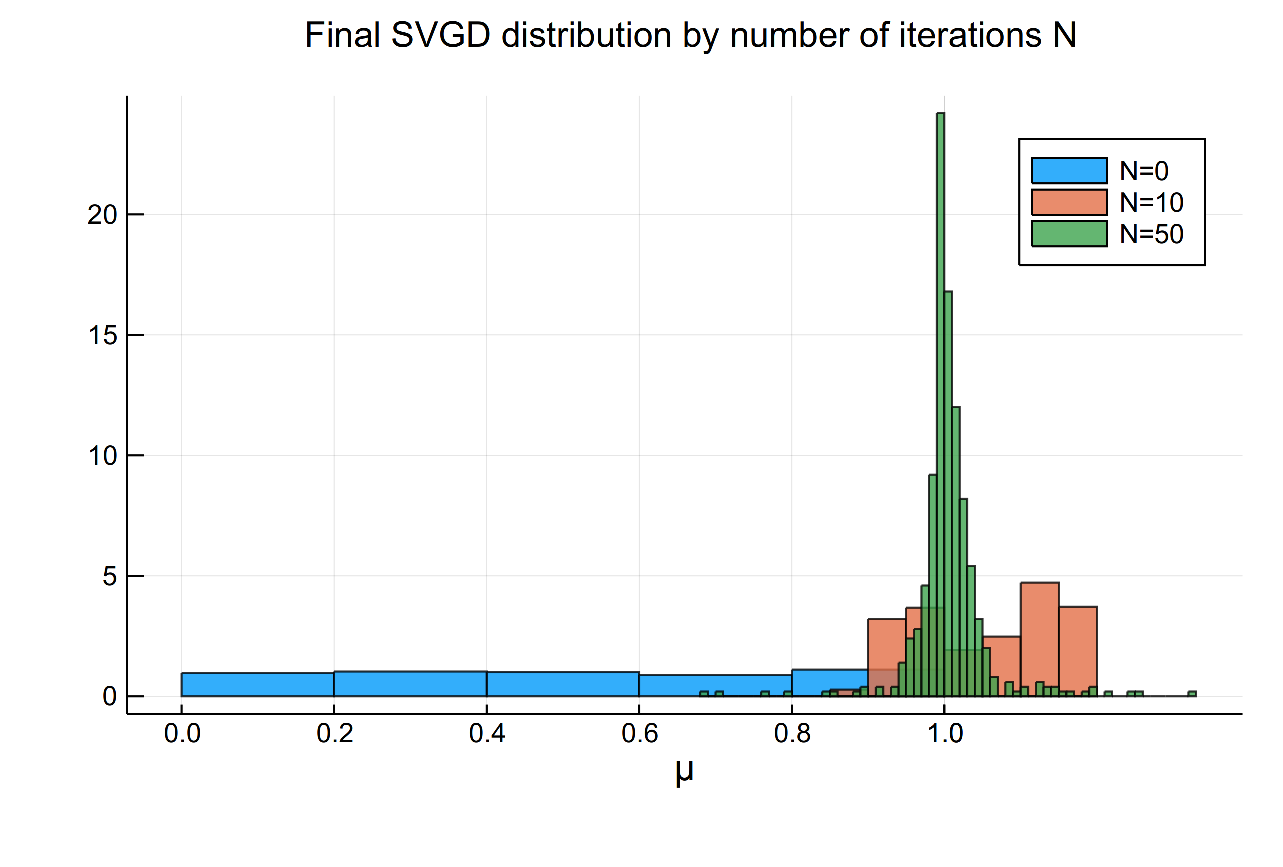
\includegraphics[width=4in]{images/svgd-example.eps}
	\caption[SVGD distribution example for different iterations.]{Graph showing how a particle distribution of 500 particles progresses towards the true parameter values of a Gaussian with mean 1. The optimisation is plotted for different amounts of iterations; the blue histogram is the initial random distribution, the green is the final result, and orange an intermediate result.}
    \label{fig:svgd-example}
\end{figure}

\begin{figure}
	\centering
	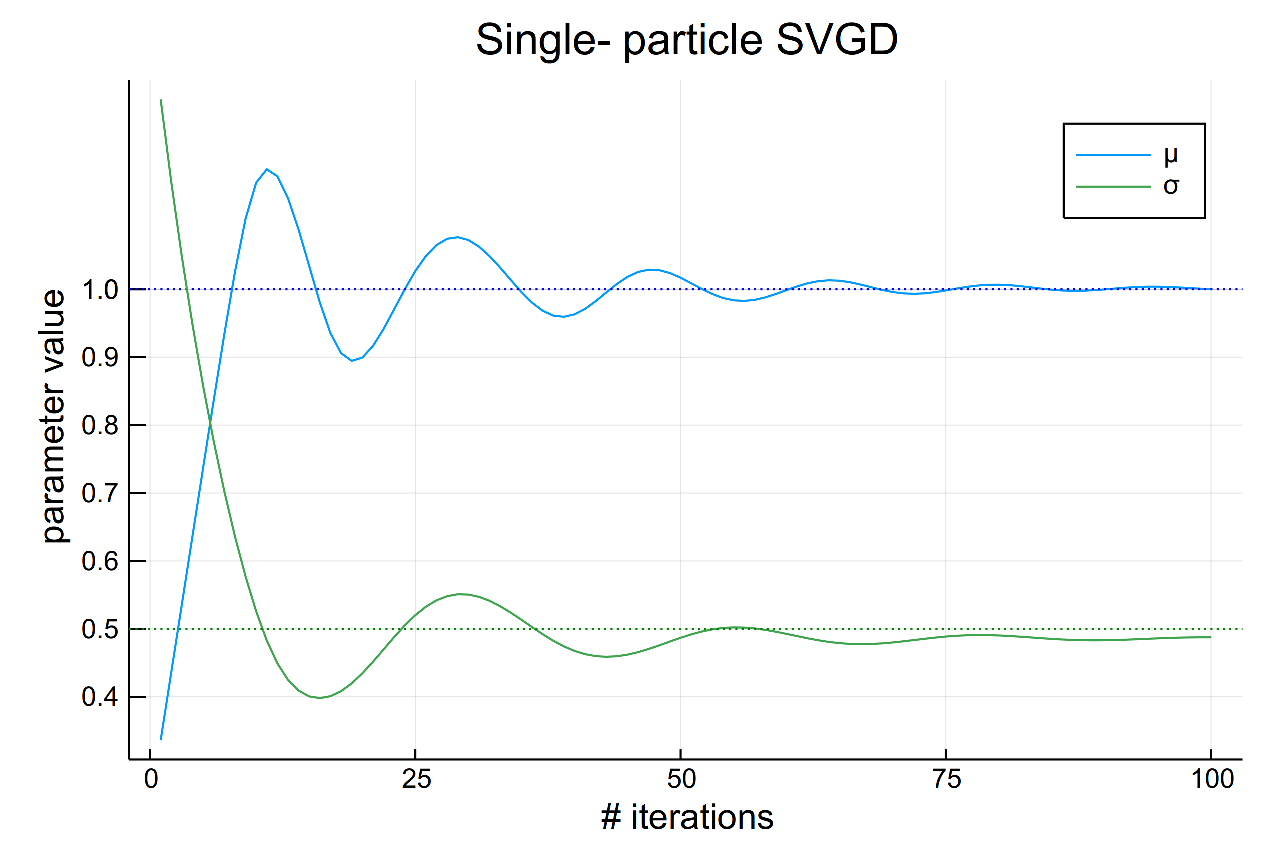
\includegraphics[width=5in]{images/svgd-map.eps}
	\caption[SVGD single-particle example graph.]{Example of the oscillating convergence of parameters $\mu$ and $\sigma$ of a Gaussian, where the dotted lines in the graph are the true parameter values. Theoretically this single-particle SVGD corresponds with MAP.}
    \label{fig:svgd-opt}
\end{figure}


\section{Comparisons of VI methods}

\subsection{Example: 1D Gaussian mixture model}
As an example we create an extremely simple Gaussian mixture model made up of two slightly overlapping normal distributions. A dataset of 1000 samples is generated with the true means $\mu_{1, 2} = (-1, 1)$ and true standard deviations $\sigma_{1, 2} = (0.3, 0.5)$.

\begin{equation}
    \begin{split}
        \mathrm{\mu}_k & \sim \mathrm{Normal}(0, 2) \\
        \sigma_k & \sim \mathrm{LogNormal}(0, 1) \\
        x_i & \sim \sum^2_{k=1} \mathrm{Normal}(\mu_k, \sigma_k) \\
    \end{split}
\end{equation}

%\begin{wrapfigure}{r}{0.5\textwidth}
\begin{figure} 
    %\begin{center}
	\centering
	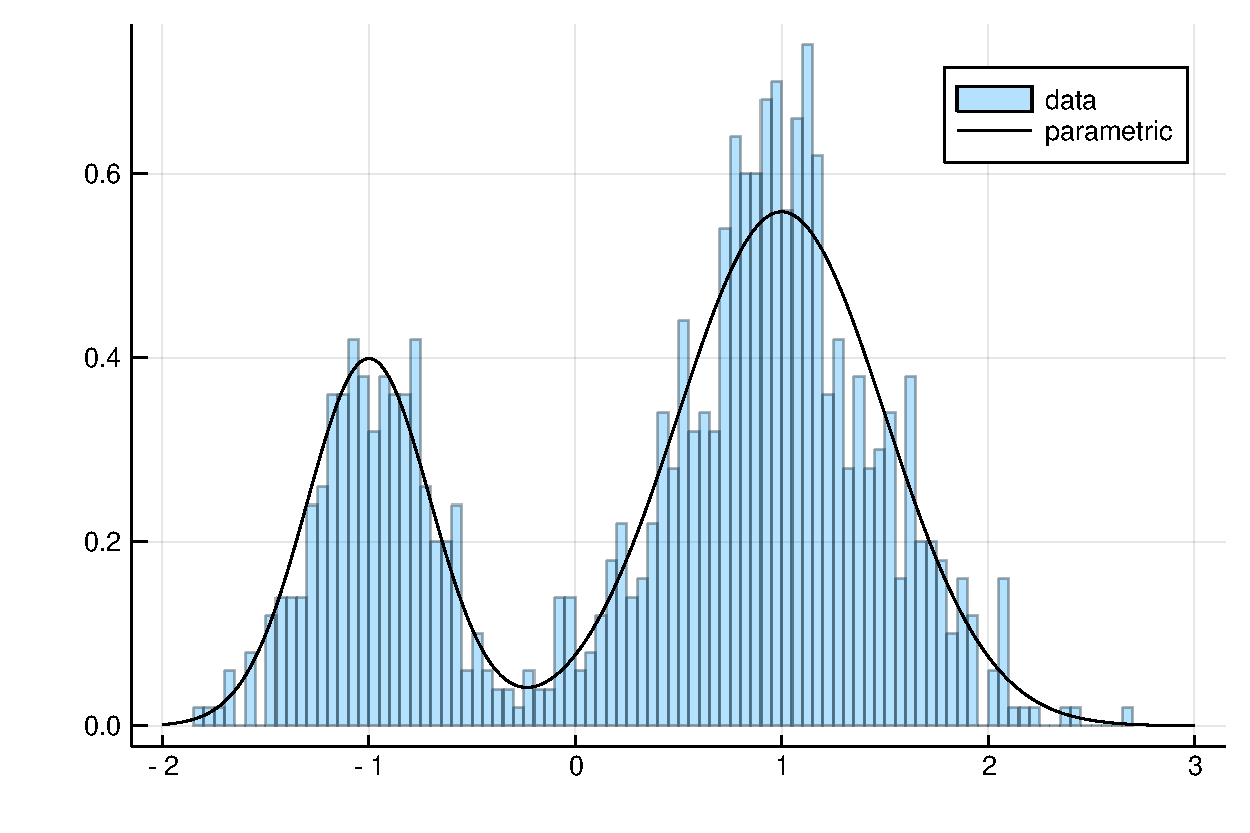
\includegraphics[width=4in]{images/vi_comp_data.pdf}
    %\end{center}
    \caption[VI comparison: true distribution of the data.]{Visualisation of the true distribution of the data samples (blue) and the parametric distribution used to generate them (black).}
    \label{fig:vi-comparison-data}
\end{figure}


    ADVI and BBVI are initialized in the same way: the initial variational distribution $q_0$ is a mean-field unit-normal distribution. Both are run for 500 iterations. 
    \\
    The 100 SVGD particles are initialized with samples from the unit normal distribution and optimised for 200 iterations. Comparison of the final distributions after optimization are visualized in Figure \ref{fig:vi-comparison}. It is clear from the graphs that all three methods find a reasonable approximation of the true values of the latent variables.
    \\ 
    In general, we note that the distributions obtained by ADVI are more narrow than the others. The parameter distributions found by SVGD are multi-modal because each particle can gravitate towards either optimum.
    

\begin{figure}
	\centering
	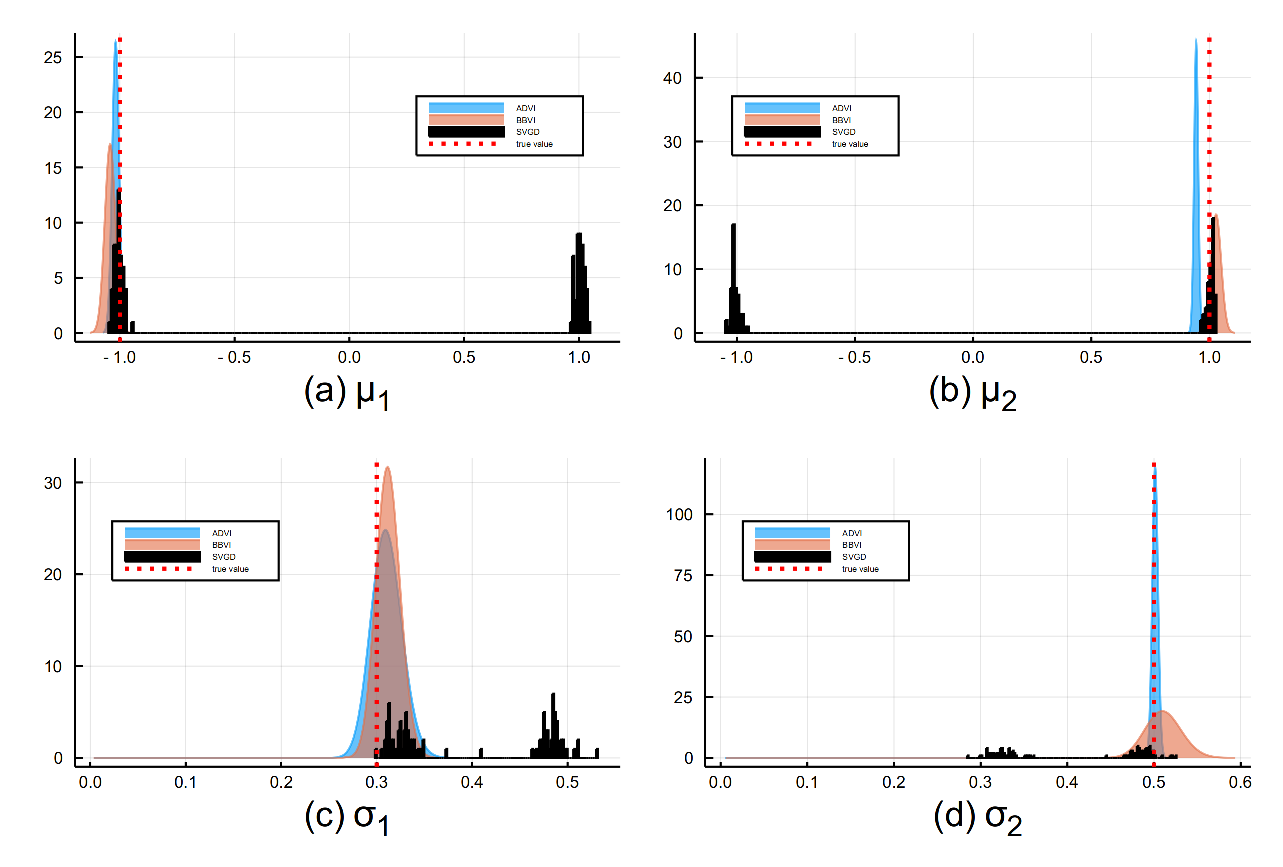
\includegraphics[width=5in]{images/vi-comp.eps}
	\caption[Comparison of densities for VI methods.]{Comparison of the inferred densities of the 1D Gaussian mixture parameters. All three methods give a reasonable approximation of the true values. Note that the results of SVGD (black) are multi-modal distributions.}
    \label{fig:vi-comparison}
\end{figure}


\subsection{Variance in gradient estimators}
BBVI and ADVI use different estimators for the gradient. Kucukelbir et al. note that the BBVI gradient estimator has much greater variance than their own ADVI method \parencite{ADVI}. When evaluating the variance for our Gaussian mixture example it is clear that this is indeed the case (see Figure \ref{fig:vi-variance}). The addition of control variates to the BBVI predictor (BBVI-CV) greatly reduces variance but it remains an order of magnitude larger than for ADVI.

\begin{figure}
	\centering
	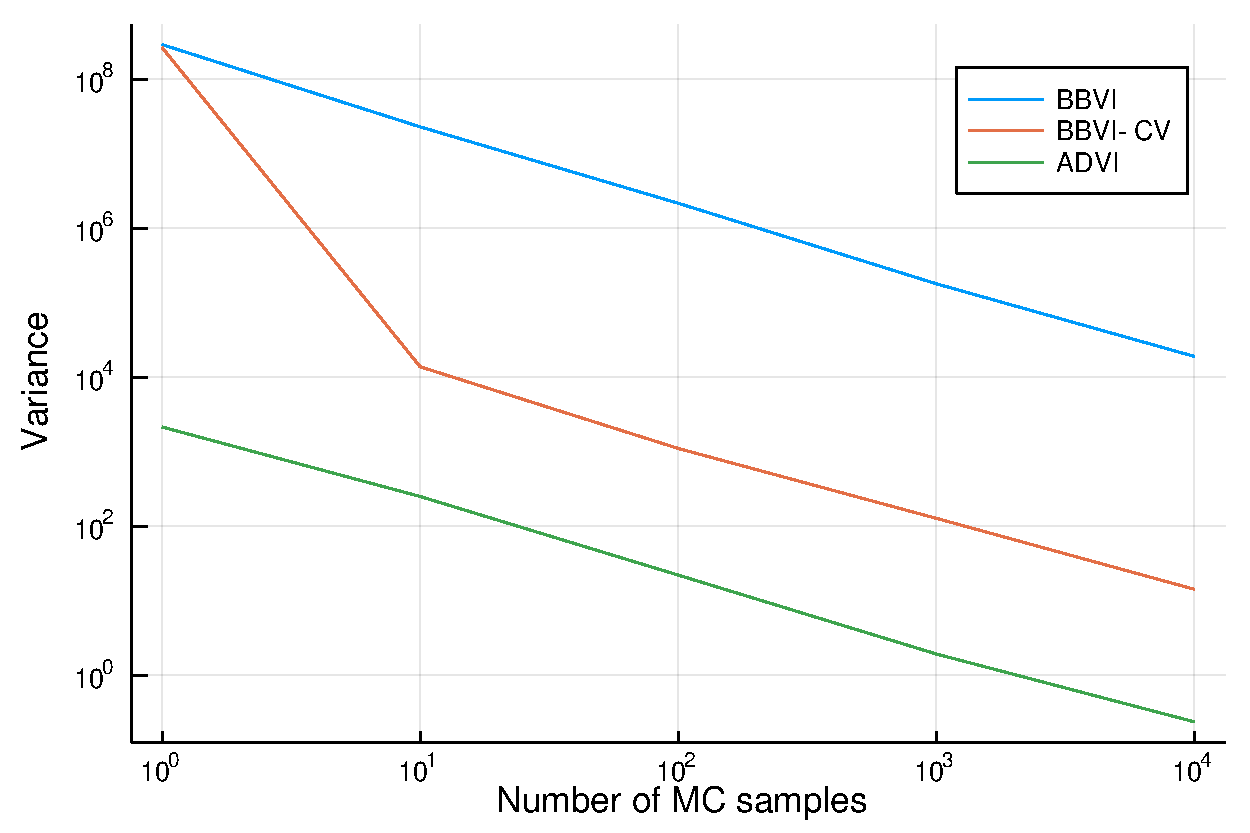
\includegraphics[width=4.2in]{images/variance_plot.pdf}
	\caption[Variance comparison of BBVI and ADVI.]{Comparison of variance on the gradient estimators of BBVI and ADVI for different amounts of Monte Carlo samples. While variance of BBVI is greatly reduced with the use of control variates (BBVI-CV), the variance of the ADVI estimator is still considerably lower.}
    \label{fig:vi-variance}
\end{figure}


\subsection{Discussion}
The results from this simple example corroborate the findings of Kucukelbir et al.: the variance of ADVI is much smaller than BBVI, resulting in much narrower peaks (Figure \ref{fig:vi-comparison}).
\\
It is also important to note that the distribution of the SVGD particles is not restricted to any variational family and that the algorithm can find multi-modal solutions when they are not expected, as in the example above. This can be useful if the shape of the distribution is completely unknown \textit{a priori}, but can make interpretation of results more difficult. An approximation that correctly estimates the mean values is often considered sufficiently accurate, which is why the mean-field normal family is most commonly used in practice \parencite{vi-review}.

\section{Variational inference in bioinformatics literature}

There have been several recent bioinformatics papers published where the authors apply variational methods to perform Bayesian inference.

\subsection{CAT model \parencite{cat}}
A variant of gradient-based variational inference called stochastic variational inference (SVI, \cite{svi}) has been successfully applied to the CAT model, which describes site heterogeneity of the nucleotide substitution process. This VI implementation proved to be up to 5x faster than MCMC and approximated the MCMC distribution accurately.

\subsection{Phylostan \parencite{phylostan}}
The \textit{phylostan} package is an extension for the probabilistic programming language Stan \parencite{Stan} that implements several common phylogenetic models. The phylostan authors opted to use the BBVI implementation already available in Stan, and compared it to the original MCMC implementation of their phylogenetic inference. They conclude that VI is much faster than MCMC, but that it is less accurate; which is what \cite{vi-review} also noted in their review paper.






\part{Experiments}

\chapter{Aims}

\section{Introduction}
In this thesis we wish to demonstrate the usefulness of the variational approach to Bayesian inference. We aim to show that variational algorithms can provide approximate solutions that approach the accuracy of the MCMC methods that are traditionally used.
\medskip 
\par The following chapter contains the computational experiments that were performed to affirm that variational inference is indeed applicable in practical phylogenetic studies. First a simulated dataset of gene counts is studied with the Beluga phylogenetic model \parencite{beluga}. Doing so, we will infer the duplication and loss rates in each branch of a plant species tree of 9 species. Following this, the same process will be performed on several real-world datasets. A dataset of closely-related rice species is studied as an example of a real analysis. We also show that the variational method can be applied to much larger species trees than is traditionally possible with MCMC by performing an analysis on 44 species from the PLAZA 4.0 dicot dataset \parencite{PLAZA-paper-1}.
\medskip
\par Finally, in Section \ref{sec:whale} we demonstrate that variational inference is applicable to another example of a state-of-the-art phylogenetic model, namely the Whale model \parencite{whale} which we will use to infer whole genome duplications in the history of a plant species tree. This is a more complex model and as such is slower. This makes it a good candidate for variational inference since any speedup here would make a big difference for end users.

\section{Acknowledgements}
Several notable contributions were made by thesis supervisor Arthur Zwaenepoel, including the supplying of phylogenetic data and help with the initial setup of the Beluga and Whale Julia libraries. He also provided several finished MCMC analyses for comparison with the VI algorithms.


\chapter{Results} \label{sec:results}

\section{Beluga simulation}

\subsection{Introduction}
\par In order to evaluate the differences between variational inference techniques (ADVI, BBVI, SVGD) and MCMC, we generate a simulated dataset where the true values are known. Doing so, it becomes possible to check not only that the different techniques reach the same final results, but also whether any inference method actually correctly estimates the ground truth.
\medskip
\par First we study the inference of the duplication ($\bm\lambda$) and loss ($\bm\mu$) rates for each species tree branch. Note that there is also a global parameter $\eta$ (which models the probability of a multiple ancestral genes at the root) for the whole tree that has to be inferred. The species tree used in this experiment contains nine plant species (see Figure \ref{fig:plants-tree}). Because this experiment is a simulation, this will be the only time in this chapter where we have access to ground truth values.

\subsection{Beluga simulation}

A Beluga model with a certain set of parameters ($\bm\lambda$, $\bm\mu$, $\eta$) was created and used to generate 500 simulated samples of gene counts. These were then randomly subsampled into mini-batches of 200 samples for the variational inference methods, while MCMC used the full dataset each iteration.
\medskip
For this simulation the inference algorithms are set up up as follows:
\begin{itemize}
    \item ADVI uses 1 MC sample and mini-batches of 200 samples. The algorithm is run for 1000 iterations.
    \item BBVI uses 10 MC samples and mini-batches of 200 samples. The algorithm is run for 1000 iterations. The variational family used here is the same mean-field distribution as used in ADVI.
    \item MCMC is run for 5000 iterations, of which 1000 are burn-in samples
    \item SVGD uses 50 particles and is run for 500 iterations with mini-batches of 50 samples.
\end{itemize}

\begin{figure}
	\centering
	\includegraphics[width=7in]{images/trees/plants-tree.png}
	\caption[Species tree for simulated plant data.]{Species tree for the plant species in the Beluga simulation study.}
    \label{fig:plants-tree}
\end{figure}


\subsubsection{Comparison of VI convergence}
Before comparing variational inference with MCMC, the optimisation of the different variational algorithms can be compared. The convergence process of the various model parameters are shown in Figures \ref{fig:beluga-sim-opt-lambda} and \ref{fig:beluga-sim-opt-mu}. It is clear that both ADVI and BBVI algorithms do not converge to the ground truth values in all cases, but we shall see that the more accurate MCMC algorithm also doesn't exactly find all of the parameters.

\medskip
\par When plotting the progress of the ELBO function, it is clear that BBVI converges faster than ADVI. While the BBVI gradient estimator is more noisy than ADVI, the rolling average of the ELBO that is shown in Figure \ref{fig:score} appears no more noisy than that of ADVI.

\begin{figure}
	\centering
	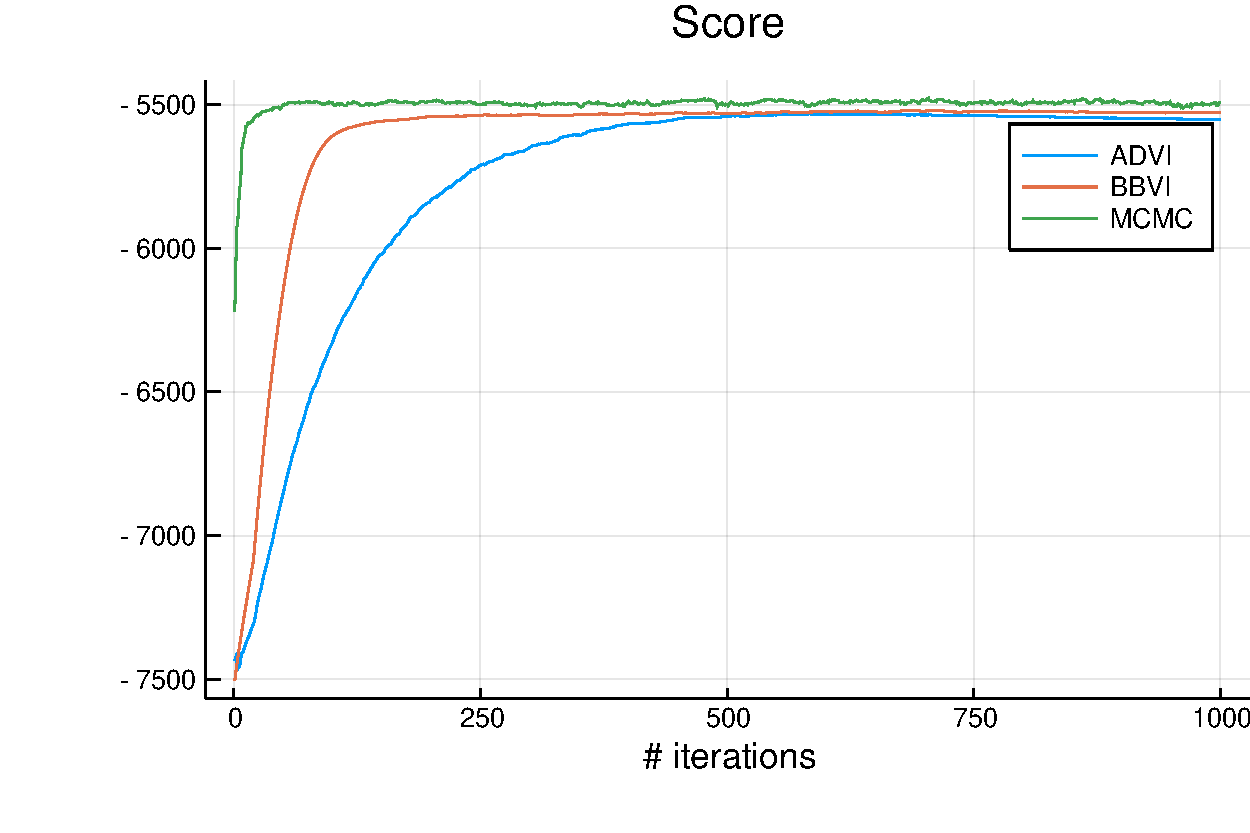
\includegraphics[width=4in]{images/simulations/beluga-sim-score.pdf}
	\caption[Beluga simulation: VI optimisation comparison]{Comparison of score functions between VI methods ADVI and BBVI, which use the ELBO as score (rolling average over 20 iterations), and the MCMC, which uses the joint likelihood. because they use different score functions the VI methods cannot be directly compared to the MCMC.}    
	\label{fig:score}
\end{figure}

\begin{figure}
	\centering
	\noindent\makebox[\textwidth]{
	    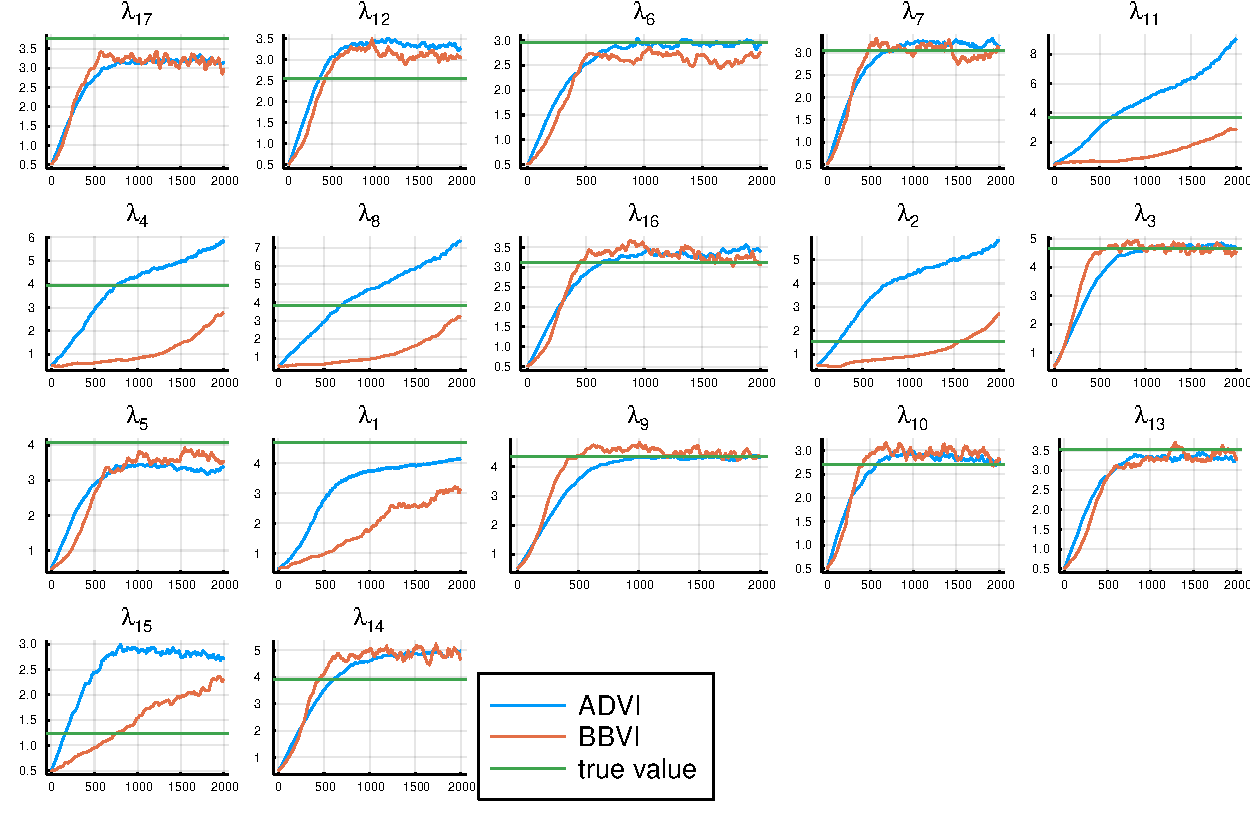
\includegraphics[width=7.5in]{images/simulations/convergence-lambda.pdf}
    }
	\caption[Beluga simulation: VI optimisation comparison for $\lambda$.]{Plots of the variational optimisation process of the variational parameter $\bm\mu$ which models the duplication rates $\bm\lambda$. Each plot shows the duplication rate for a different branch in the species tree. Both BBVI (red) and ADVI (blue) are shown in relation to the ground truth values (green).}
    \label{fig:beluga-sim-opt-lambda}
\end{figure}

\begin{figure}
	\centering
	\noindent\makebox[\textwidth]{
	    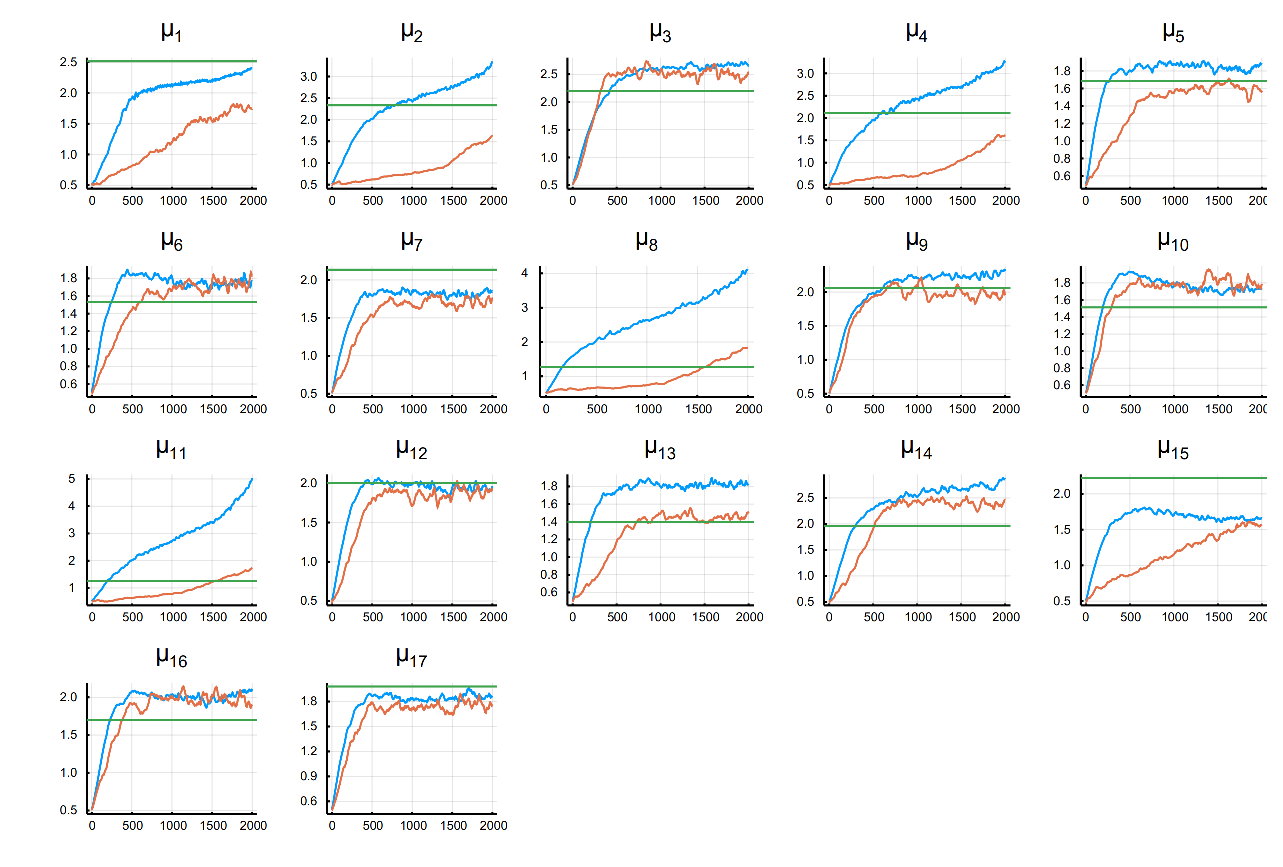
\includegraphics[width=7.5in]{images/simulations/convergence-mu.eps}
	}
	\caption[Beluga simulation: VI optimisation comparison for $\mu$.]{Plots of the variational optimisation process of the variational parameter $\bm\mu$ which models the loss rates $\bm\mu$. Each plot shows the loss rate for a different branch in the species tree. Both BBVI (red) and ADVI (blue) are shown in relation to the ground truth values (green).}
    \label{fig:beluga-sim-opt-mu}
\end{figure}


\subsubsection{Comparison with MCMC}
The approximate VI distributions for each latent model parameter can be compared to the distribution of the MCMC trace (Figures \ref{fig:beluga-sim-distribution-lambda}, \ref{fig:beluga-sim-distribution-mu}). It is immediately evident from the figures that none of the methods find the all the correct parameter values, not even MCMC which is expected to be the most accurate.
\\
While both VI methods provide reasonable approximations, it is clear that the variational distribution of BBVI (blue in Figures \ref{fig:beluga-sim-distribution-lambda} and \ref{fig:beluga-sim-distribution-mu}) more exactly matches the posterior found by MCMC. While ADVI has a very similar mean, the distribution is often too narrow. In practice we notice that the variational parameters for the variance ($\bm\omega$) of ADVI do not change much from the starting values, so a correct initial estimate is paramount; BBVI suffers from the same problem to a lesser extent.
\\
SVGD (with 50 particles) is plotted separately against MCMC to avoid cluttering in the plot (see Figure \ref{fig:beluga-sim-svgd}). We provide only the duplication rates here because this is sufficient to see that SVGD does not provide anywhere near the accuracy of BBVI or ADVI; there are several branches where the algorithm completely misses the target which does not happen with the other two VI methods.



\begin{figure}
    \noindent\makebox[\textwidth]{
	    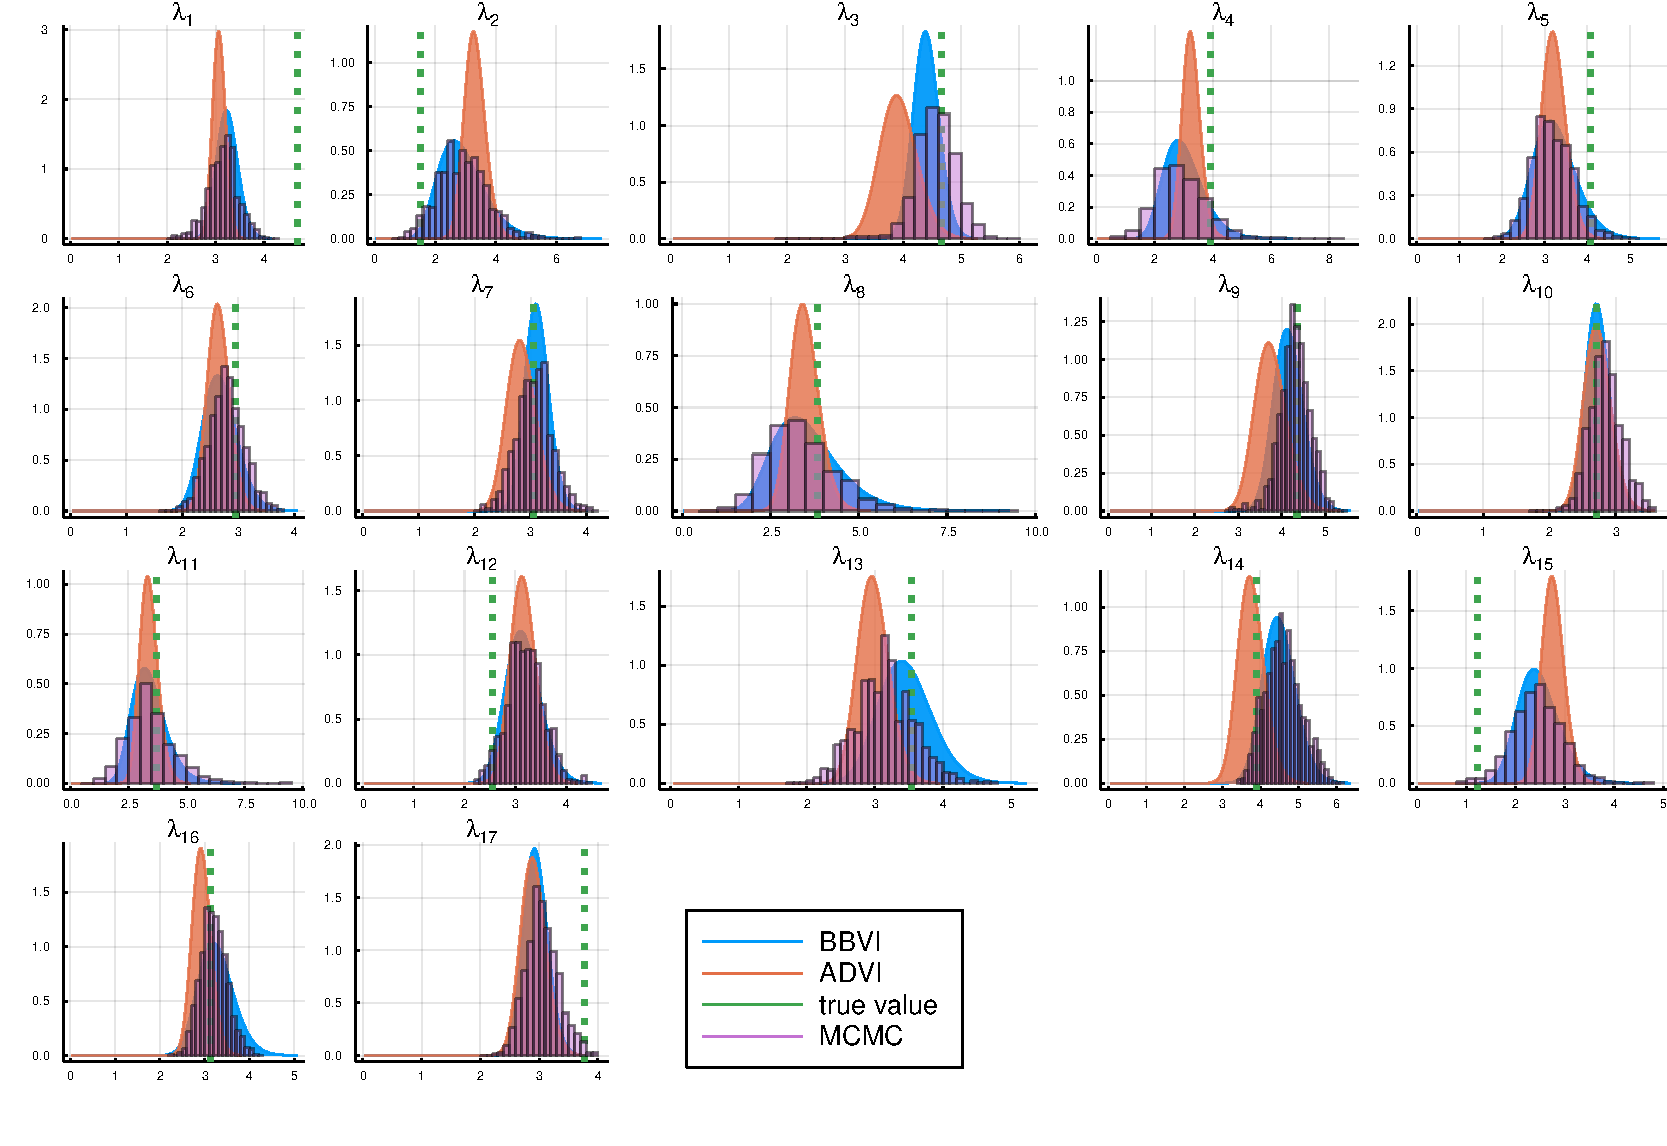
\includegraphics[width=7in]{images/simulations/beluga-sim-distribution-lambda.pdf}
	}
	\caption[Beluga simulation: VI approximation and MCMC comparison]{A comparison of the variational approximations and MCMC for the $\lambda$ parameters of the Beluga model on a simulated dataset. The approximations for ADVI (orange), BBVI (blue) are compared with MCMC (pink) and the ground truth values of the simulation (green).}
    \label{fig:beluga-sim-distribution-lambda}
\end{figure}

\begin{figure}
    \noindent\makebox[\textwidth]{
	    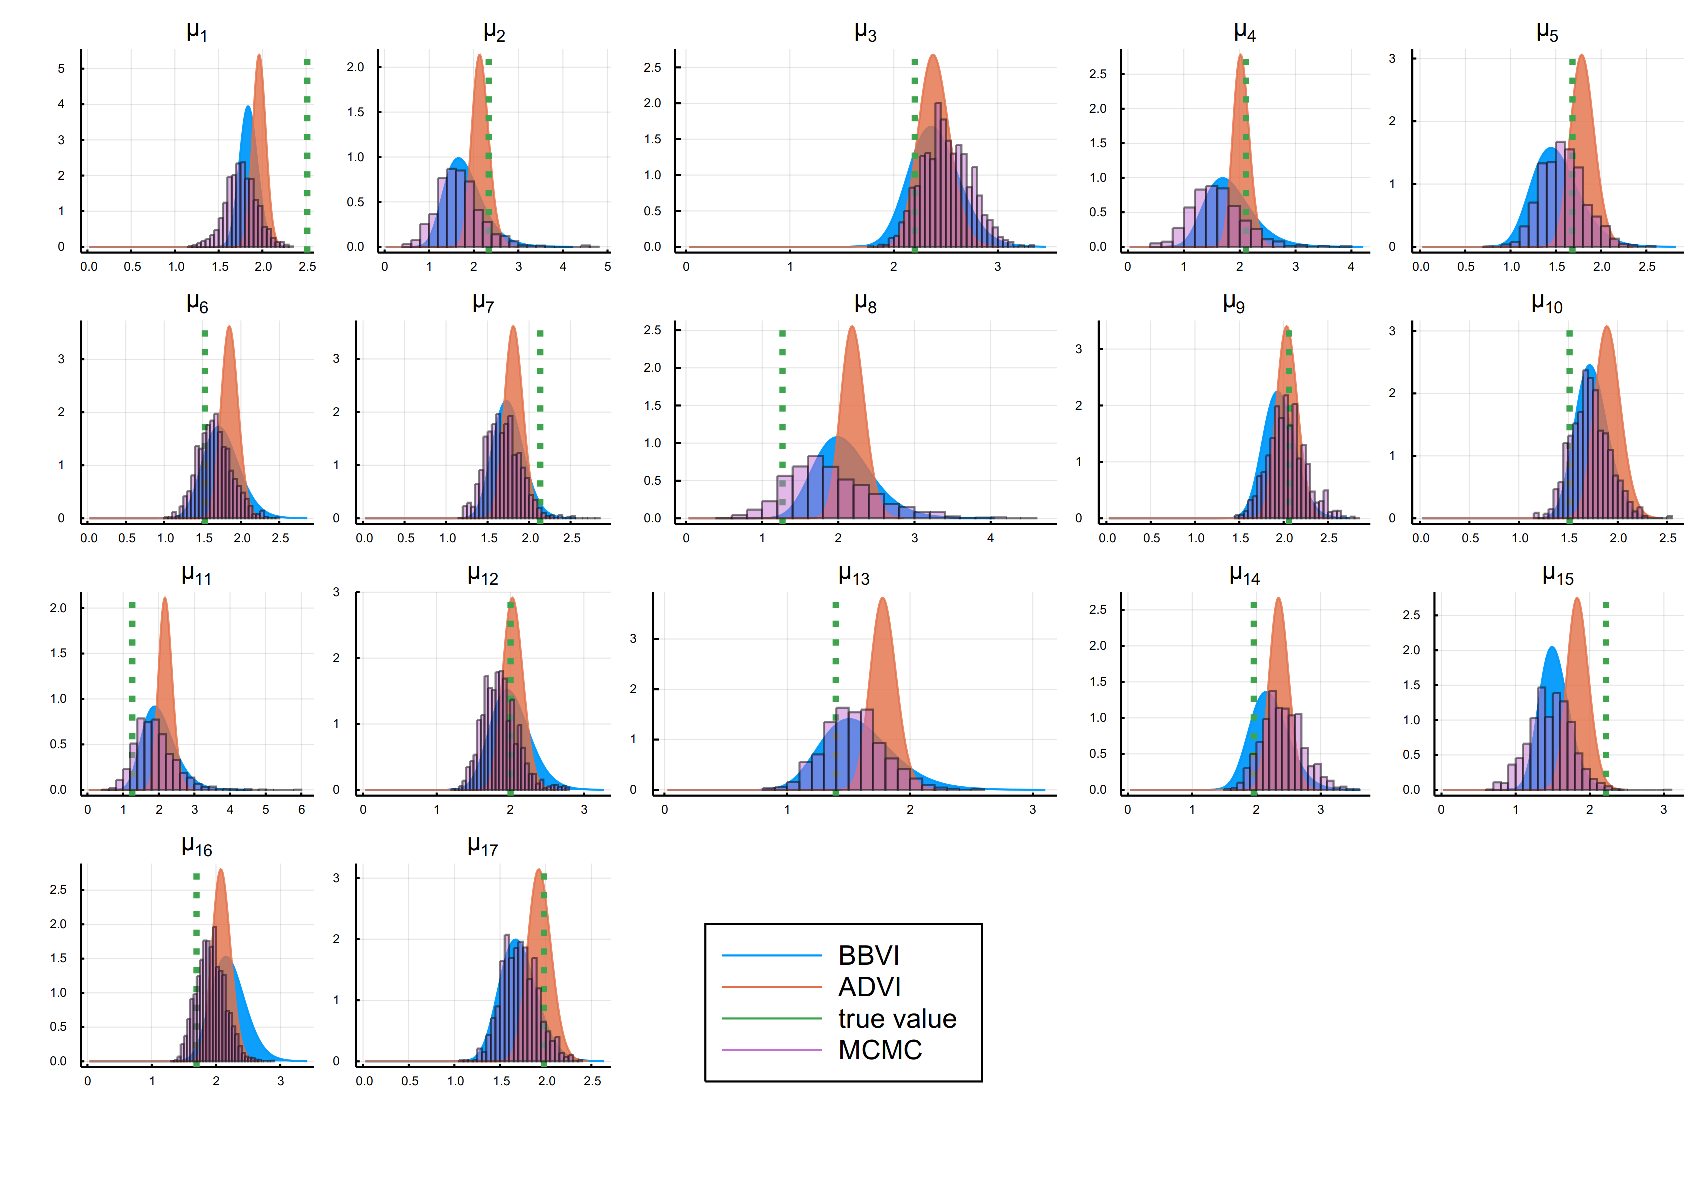
\includegraphics[width=7in]{images/simulations/beluga-sim-distribution-mu.eps}
	}
	\caption[Beluga simulation: VI approximation and MCMC comparison]{A comparison of the variational approximations and MCMC for the $\mu$ parameters of the Beluga model on a simulated dataset. The approximations for ADVI (orange), BBVI (blue) are compared with MCMC (pink) and the ground truth values of the simulation (green).}
    \label{fig:beluga-sim-distribution-mu}
\end{figure}

\begin{figure}
    \noindent\makebox[\textwidth]{
	    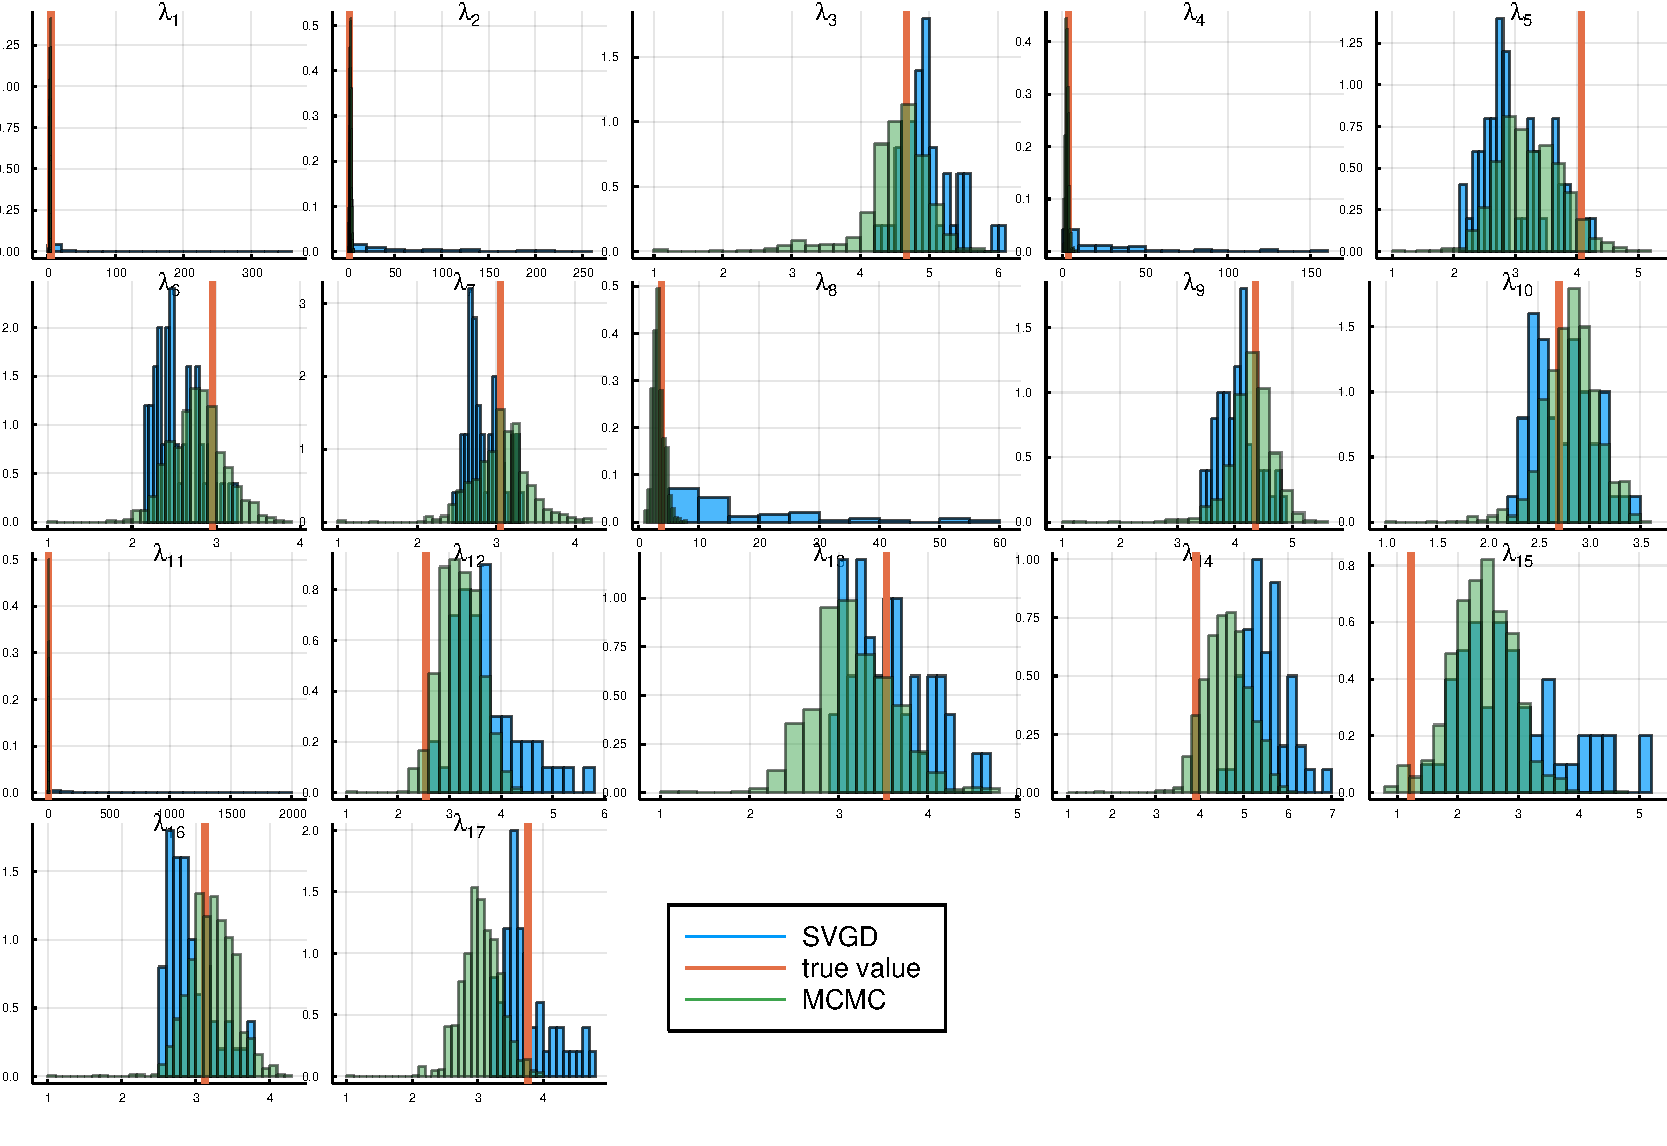
\includegraphics[width=7in]{images/simulations/beluga-sim-distribution-mu.pdf}
	}
	\caption[Beluga simulation: VI approximation and MCMC comparison]{A comparison of the variational approximations and MCMC for the $\lambda$ parameters of the Beluga model on a simulated dataset. The approximations for ADVI (orange), BBVI (blue) are compared with MCMC (pink) and the ground truth values of the simulation (green).}
    \label{fig:beluga-sim-svgd}
\end{figure}

\subsubsection{Time analysis}
While variational inference is known to be less accurate than MCMC - it is always an approximate solution - the advantage of VI cited in the literature \parencite{vi-review} is that it is faster. Our simulation experiment confirms this: both VI methods are indeed considerably faster. Among the different variational methods tested, BBVI is clearly the fastest. 
\\
This is likely because the models studied in this thesis have very expensive model gradients, which means that the methods which use this gradient (ADVI, SVGD) are at a disadvantage here when it comes to computational time. These methods will be more competitive when the model gradient $\nabla\mathrm{log}p(\bm x, \bm\theta)$ is not much more expensive than the model density $\mathrm{log}p(\bm x, \bm\theta)$ as is the case here.
\\
SVGD typically uses at least 50 particles, which in this case would be much slower than the MCMC. For being slower than the gold standard, we will discard SVGD in the rest of the experiments in this chapter and only continue comparing ADVI, BBVI and MCMC.



\begin{table}[]

    \caption[Beluga computation time benchmarks]{Computation time benchmarks for the Beluga simulation data. ADVI and BBVI use 1 and 10 Monte Carlo samples respectively, and al VI methods use mini-batches of 100 samples. A full analysis consists of 1000 iterations for ADVI, SVGD and BBVI, and 5000 iterations for MCMC.}
    \centering
    \begin{tabular}{l||lllll|}
    \cline{2-5}
     & \multicolumn{4}{c|}{\textbf{Inference method}}                                                                            \\ \hline
    \multicolumn{1}{|l||}{\textbf{\# iterations}} & \multicolumn{1}{l|}{ADVI} & \multicolumn{1}{l|}{BBVI}  & \multicolumn{1}{l|}{SVGD-50} & MCMC \\ \hline
    \multicolumn{1}{|l||}{1}                      &         1.08s             &          \textbf{0.48s}               &            3.83s                 &                                 0.56s   \\ \hline
    \multicolumn{1}{|l||}{10}                     &         11.52s            &           \textbf{4.12s}                &          43.1s           &                       6.70s \\ \hline
    \multicolumn{1}{|l||}{full analysis}          &         1103.2s                  &     \textbf{389.9s}         &     4074.95s                &                                 3476.9s   \\ \hline
    \end{tabular}
    \label{tab:time-sim}

\end{table}


\section{Beluga with real-world data}

\par The previous section described a comparison of the variational approaches with traditional MCMC sampling on a synthetic dataset generated with the Beluga model. This section contains similar comparisons but for problems with real-world datasets. 


\subsection{Beluga rice dataset}

\par Now we present a study of the phylogenetic relationship between more closely related plant species. High-quality gene count data is available for different species of rice which have a common ancestor estimated at $\sim$15 Mya. A species tree is reconstructed from a figure available in the original paper (\cite{rice}, Figure 1.b), where \textit{L. perrieri} is added as an outgroup to the rice species. Since these species are very closely related, we do not expect much activity in the branches. Both the duplication and loss rates should be small.

\begin{comment}
Because the rice species are closely related, we do not expect to find evidence of a whole genome duplication event within the rice. It is, however, widely accepted that a WGD event occurred shortly before the speciation event in the common ancestor of rice ($\sim$20 Mya) \parencite{rice-split}.
\end{comment}

\begin{comment}
\subsubsection{Preprocessing}
Gene families that did not have at least one gene in the \textit{L. perrieri} branch were filtered out. Typically gene families are also further filtered on size as extremely large and extremely small families are removed from the data.
\end{comment}

\subsubsection{Results analysis}
It is very clear in this case that VI is much faster: running the MCMC algorithm for 10,000 iterations (of which 1000 burn-in) takes several hours (430.8 min), while the ADVI and BBVI algorithms converge in less than an hour (30.2 min and 23.8 min respectively).
\medskip
\par The results are similar to the simulation study, in that we find BBVI to be most like the MCMC results, with ADVI showing results that deviate somewhat more. We find that many branches have duplication and loss rates that are nearly zero, which is expected since these rice species are all close relatives.

\begin{figure}
	\centering
	\includegraphics[width=6.5in]{images/trees/rice-species-tree.png}
	\caption[Species tree of rice dataset]{Species tree of the rice dataset, containing 10 species of rice and \textit{Leersia perrieri} as an outgroup. Also see Figure 1.b in Stein et al. \parencite{rice}.}
    \label{fig:rice-tree}
\end{figure}

\begin{figure}
    \noindent\makebox[\textwidth]{
	    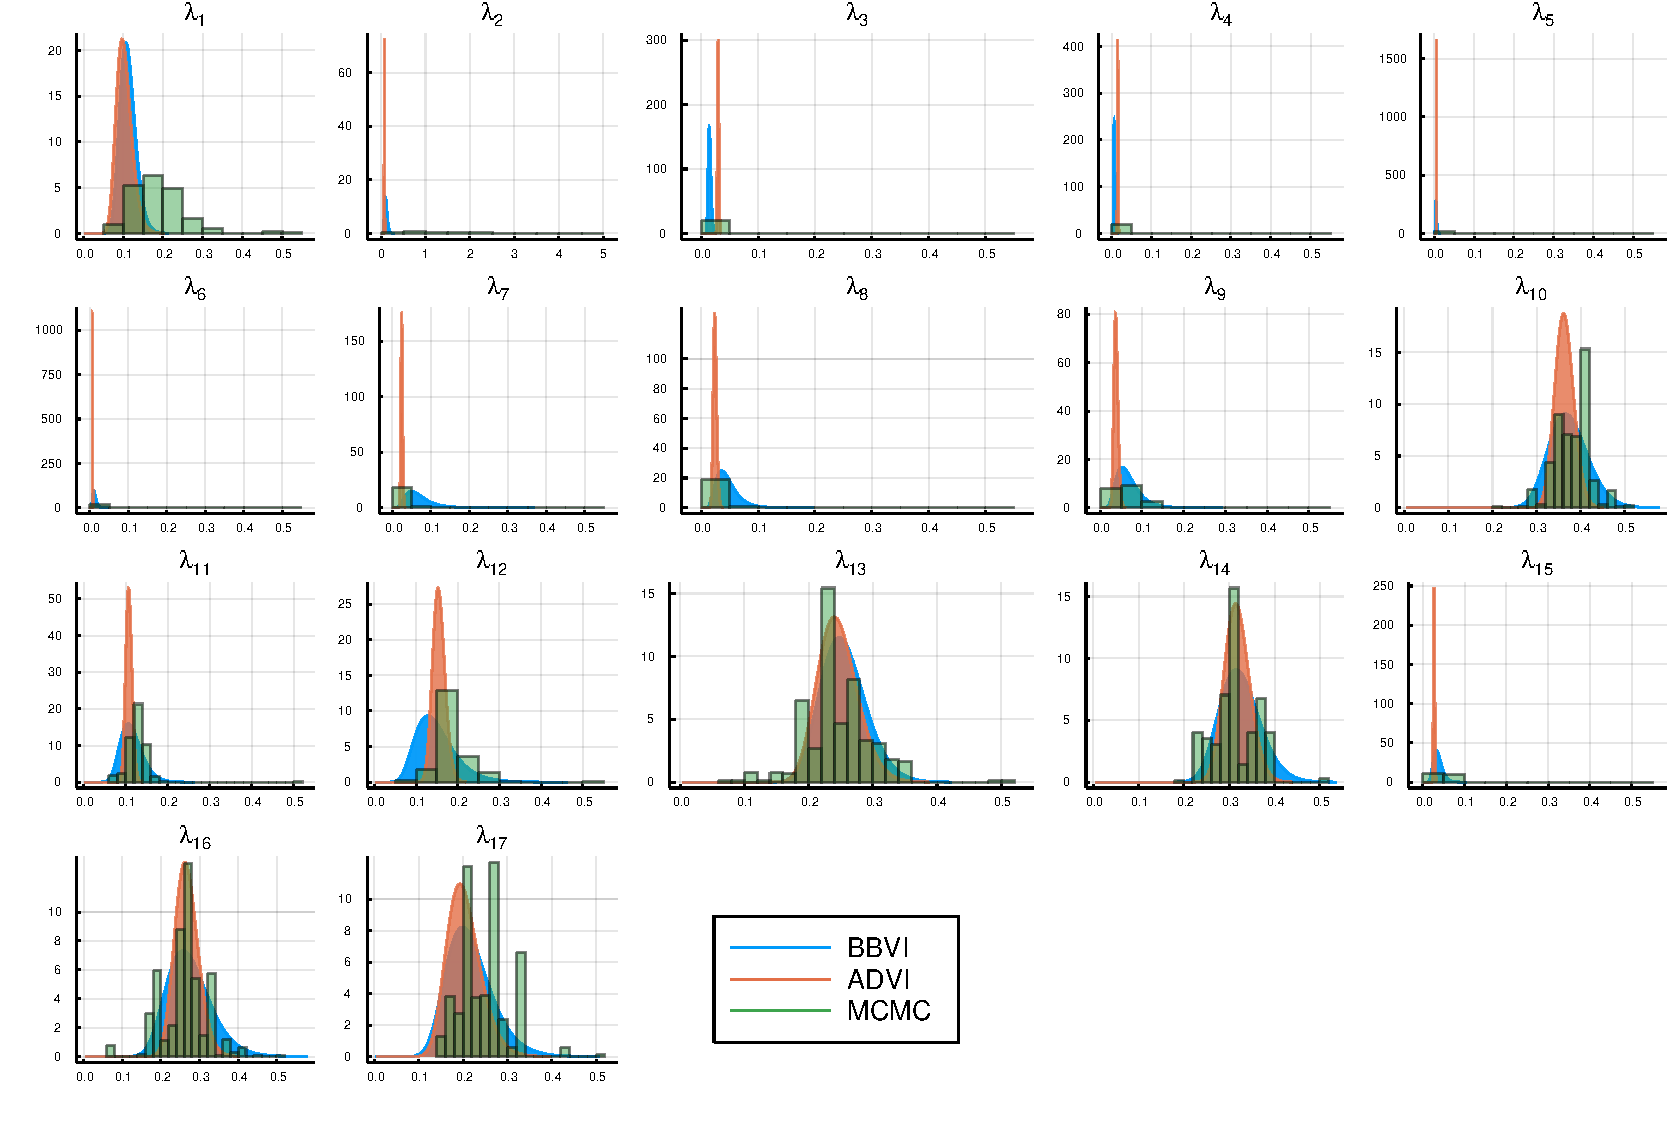
\includegraphics[width=7.2in]{images/rice/rice-lambda.pdf}
	}
	\caption[Rice Beluga duplication rates]{Overview of the distributions of the duplication rates $\lambda$ in each branch for the Beluga analysis of the rice dataset.}
    \label{fig:rice-lambda}
\end{figure}

\begin{figure}
    \noindent\makebox[\textwidth]{
	    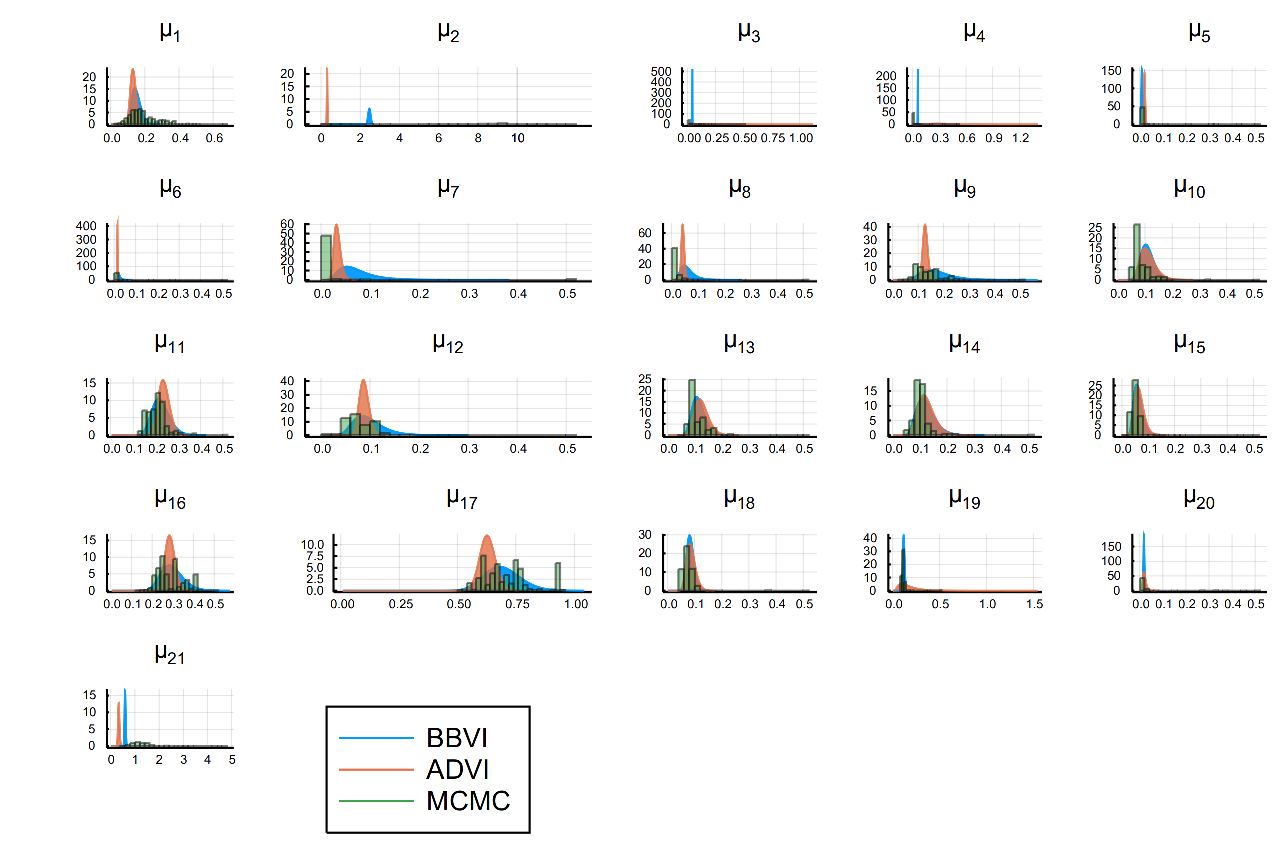
\includegraphics[width=7.2in]{images/rice/rice-mu.eps}
	}
	\caption[Rice Beluga duplication rates]{Overview of the distributions of the loss rates $\mu$ in each branch for the Beluga analysis of the rice dataset.}
    \label{fig:rice-lambda}
\end{figure}


\subsection{Beluga PLAZA dataset}

\par The PLAZA access platform \parencite{PLAZA-paper-1, PLAZA-paper-2} contains a curated set of genomic and transcriptomic data compiled from different sequencing studies. In this thesis we use a subset of the PLAZA 4.0 dicot dataset which contains 44 plant species (Figure \ref{fig:PLAZA-trees}).
\medskip
\par The PLAZA dataset is an example of a problem that cannot feasibly be solved with the existing MCMC method because it would take too long to compute. For 44 species the Beluga model contains 89 duplication rates, 89 loss rates and an additional parameter $\eta$. Variational methods are useful here because they can operate on small mini-batches of data instead of the full dataset. For computational reasons only 250 gene families were used here. BBVI was the only method tested here because it is the only method that reached a stable result; ADVI would collapse into a situation with infinite variance which crashed the optimisation process.

\begin{figure}
    \noindent\makebox[\textwidth]{
        \hspace{-2.6cm}
	    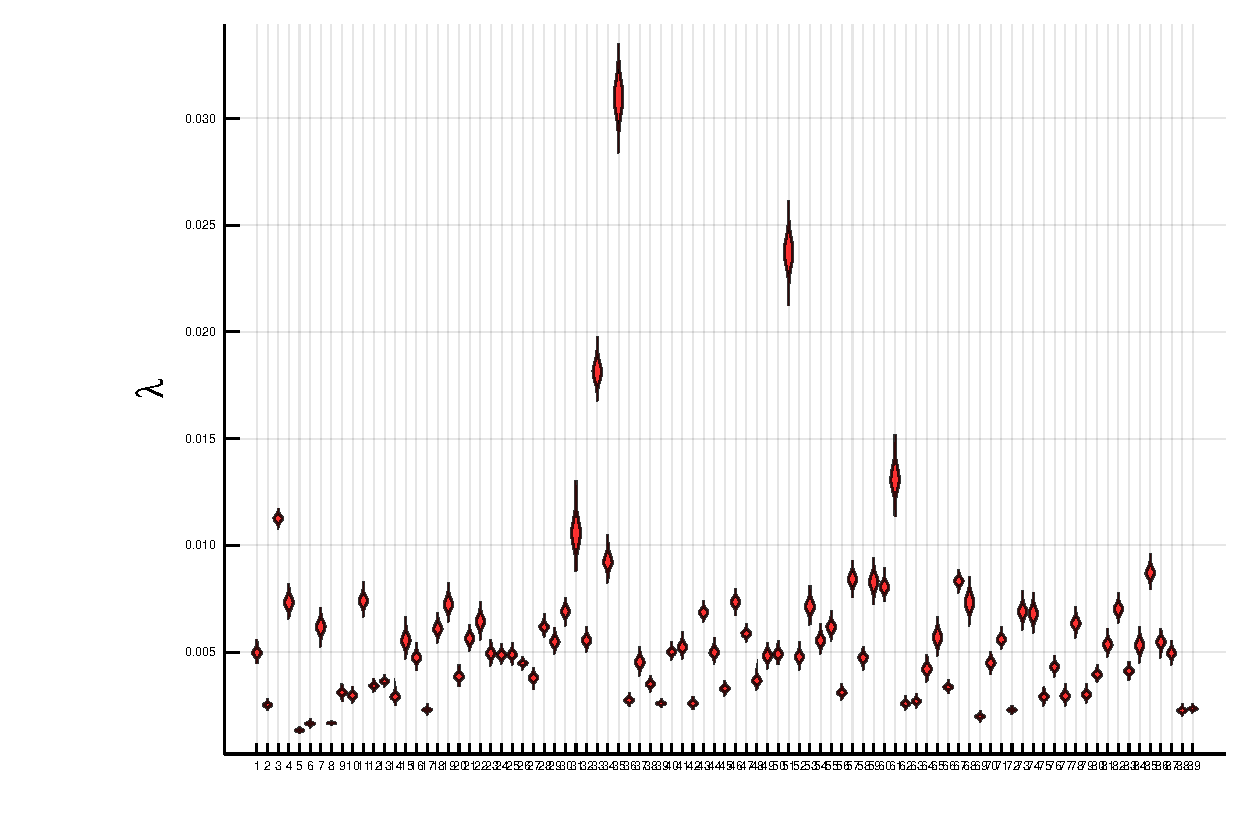
\includegraphics[width=7in]{images/PLAZA/plaza-lambda.pdf}
	}
	\caption[PLAZA Beluga duplication rates]{Overview of violin plots of the duplication rates $\lambda$ in each branch for the Beluga analysis of the PLAZA dataset.}
    \label{fig:plaza-lambda}
\end{figure}

\begin{figure}
    \noindent\makebox[\textwidth]{
        \hspace{-2.6cm}
	    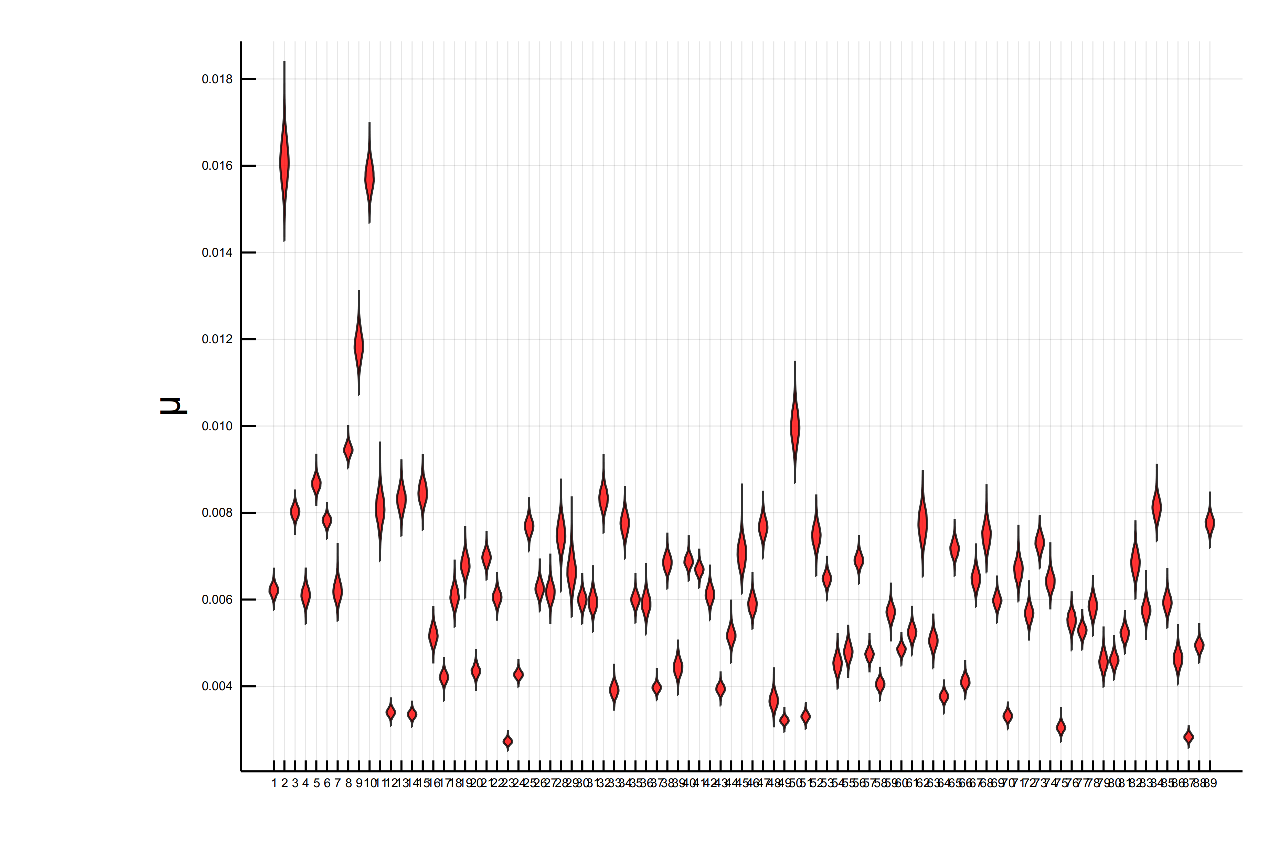
\includegraphics[width=7in]{images/PLAZA/plaza-mu.eps}
	}
	\caption[PLAZA Beluga loss rates]{Overview of violin plots of the loss rates $\mu$ in each branch for the Beluga analysis of the PLAZA dataset.}
    \label{fig:plaza-mu}
\end{figure}

\par We notice that the duplication rates (Figure \ref{fig:plaza-lambda}) and loss rates (Figure \ref{fig:plaza-mu}) are incredibly small, and there are very few outliers. Presumably this is because the branches in this species tree are, on average, much shorter than those in the smaller species trees; there is less time for events to occur. Also note that $\eta$ is tightly clustered around 0.5 in this result, so we do not have a situation where $\eta$ collapsed to zero which can sometime occur and usually indicates a faulty prior. It is unclear whether this is an abnormal result for this dataset, and should be an item for further study.

\begin{figure}
\begin{subfigure}{.5\textwidth}
  \centering
  \includegraphics[width=0.95\linewidth]{images/trees/plaza-tree.png}
  \caption{}
  \label{fig:sfig1}
\end{subfigure}%
\begin{subfigure}{.5\textwidth}
  \centering
  \includegraphics[width=0.95\linewidth]{images/trees/plaza-tree-2.png}
  \caption{}
  \label{fig:sfig2}
\end{subfigure}
\caption[Species tree of 44 PLAZA species]{Visualisations of the species tree used in the PLAZA experiment (44 species). Both the species tree with correct branch lengths (a) and a more visually clean tree with non-realistic branch lengths (b) are given. Trees were generated with iTOL \parencite{itol}.}
\label{fig:PLAZA-trees}
\end{figure}


\subsection{General notes on Beluga results}

The stochastic nature of the VI algorithms makes results strongly dependent on the initial parameter values of the variational distribution. When working on real-world data we observed that the starting values for the variational parameters must be chosen carefully and require some basic knowledge of the statistical model. The step-size parameter choice is also highly dependent on the model. In general we recommend the ADAM optimiser \parencite{ADAM} with a starting learning rate of 0.05. This learning rate should be lowered if excessive variability in the ELBO is noticed during the optimisation.
\\
We recommend the subsampling of the data into mini-batches of 100 to 200 samples since using smaller batches proved too noisy on real-world data. Conversely, using the full dataset on each iteration largely removes the speed advantage that VI has over the traditional MCMC methods.
\\
In general it appears that, of the two variational algorithms tested, BBVI is the most suitable for the Beluga model because it does not require calculation of the expensive model gradient. This means that we can use a much higher number of MC samples than ADVI and still converge faster.

\section{Whale model} \label{sec:whale}

\subsection{Introduction}
In this section we demonstrate another application of variational inference in a setting where previously only MCMC was used. The Whale library (see Methods and Materials) is another model currently in development at the VIB, and can be used to model hypothesised whole genome duplications (WGDs) in branches of the species tree \parencite{whale}. Whale uses probabilistic representations of gene trees (ALE) instead of the simple gene counts that are used in the Beluga model. As a result Whale is much slower; and a typical publishable analysis can take several days. This is an ideal candidate for variational inference because the improvement in computational speed could drastically change how analyses are performed.

\begin{figure}
	\centering
	\includegraphics[width=6.5in]{images/whale/whale-tree.png}
	\caption[Species tree of Whale experiment dataset]{Species tree used in the Whale experiment. Five hypothetical WGD nodes are placed on the species tree (black dots).}
    \label{fig:whale-tree}
\end{figure}


\subsection{Experiment}

\begin{figure}
	\centering
	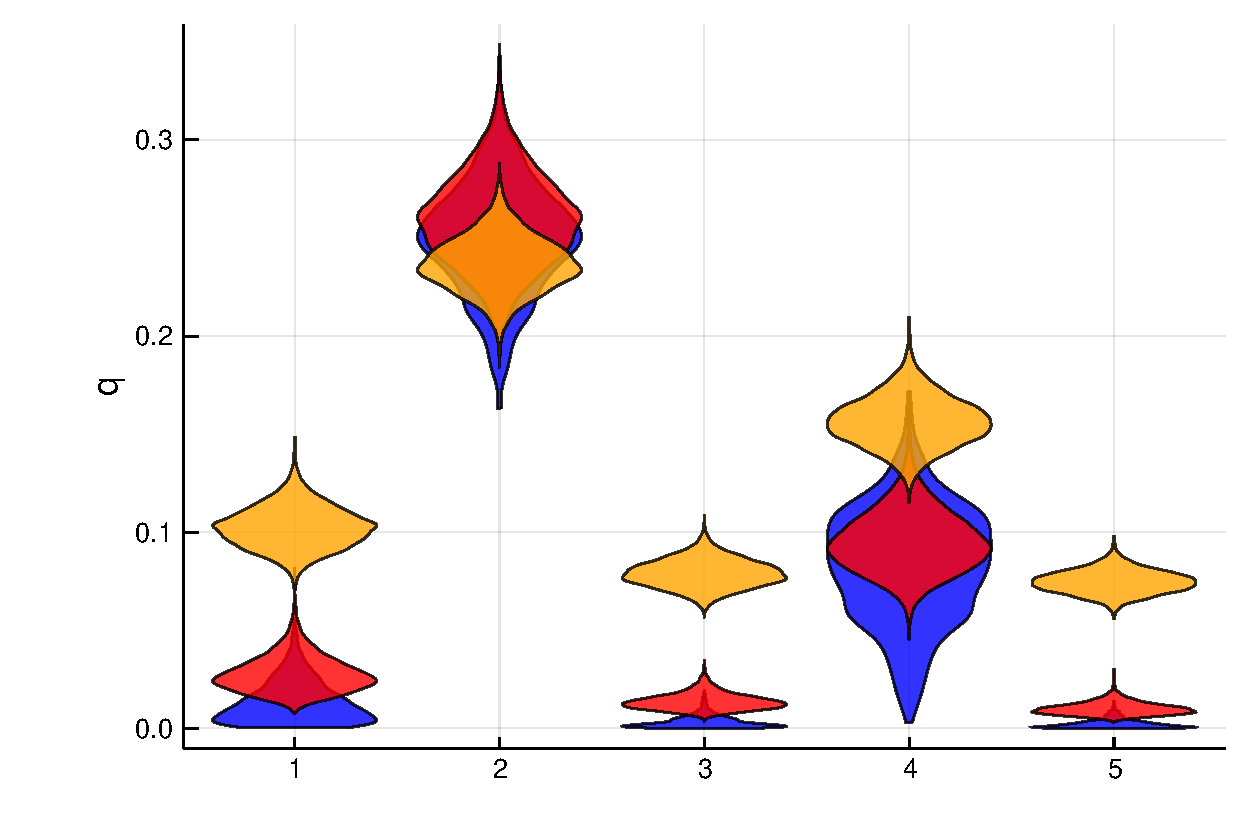
\includegraphics[width=5.2in]{images/whale/whale-q.pdf}
	\caption[Whale experiment retention rates $q$.]{Violin plots comparing the retention rates $q_i$ for the five hypothesised WGDs, with i$\, \in \{1, 5\}$. Plots are provided for the different methods of Bayesian inference: ADVI (yellow), BBVI (red) and MCMC (blue).}
    \label{fig:whale-q}
\end{figure}
\medskip
Just like the previously discussed Beluga model, Whale also models the evolutionary history of a set of species with duplication ($\lambda$) and loss rates ($\mu$), but here additional parameters $q$ are added, which model the retention of genes directly after a hypothesised WGD event.\footnote{Note that Beluga can also model whole genome duplications, we just chose not to in the previous examples.}
\medskip
\par We note that the variational methods ADVI and BBVI converge much faster here than the MCMC, which takes several hours even for a small dataset of only 500 samples. In comparison, the variational algorithms both converge in under 30 min and provide good approximations of the MCMC results.
\medskip
\par The BBVI results lead to the same conclusions as the MCMC regarding the presence of whole genome duplications in the evolutionary history of this species tree. We do not find evidence for a WGD in the branches of $q_1, \, q_3  \, or \, q_5$. There is, however, evidence for a WGD event in $q_2$. It is also evident that using ADVI here might lead to different conclusions, as ADVI finds more support a WGD in $q_4$ than the other methods.
All three methods find values closely centered around $\eta$=0.9.
\\
The resulting distributions for the duplication rates $\lambda$ and loss rates $\mu$ prove similar to the previous experiment with Beluga, in that both ADVI and BBVI give a very good approximation, but that BBVI appears on average to match MCMC slightly better.
\medskip
\par The variational solutions for the Whale are also affected by the initial parameter values.

\begin{figure}
	\centering
	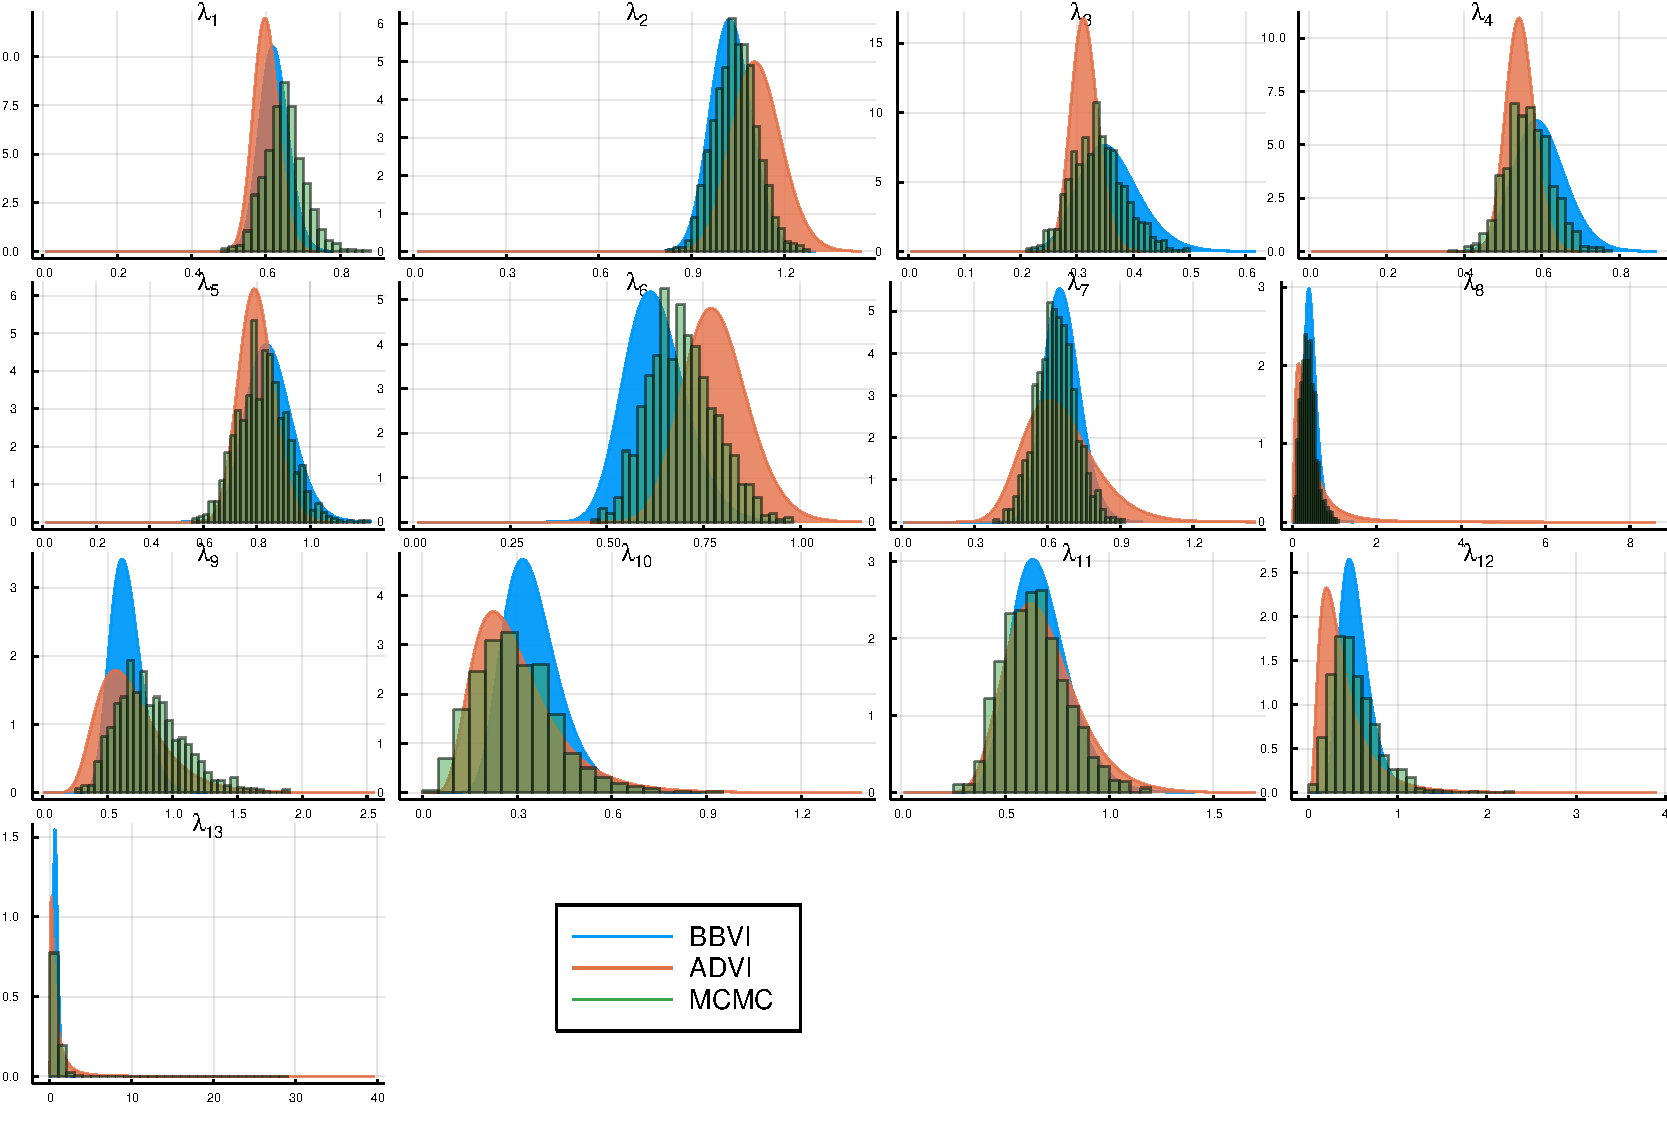
\includegraphics[width=6in]{images/whale/whale-distribution-lambda.pdf}
	\caption[Whale experiment $\lambda$ distributions.]{Comparison of different inference algorithms for the Whale model. The distributions of the different duplication rates $\lambda$ are given for BBVI (blue), ADVI (orange) and MCMC (green) respectively.}
    \label{fig:whale-lambda}
\end{figure}

\begin{figure}
	\centering
	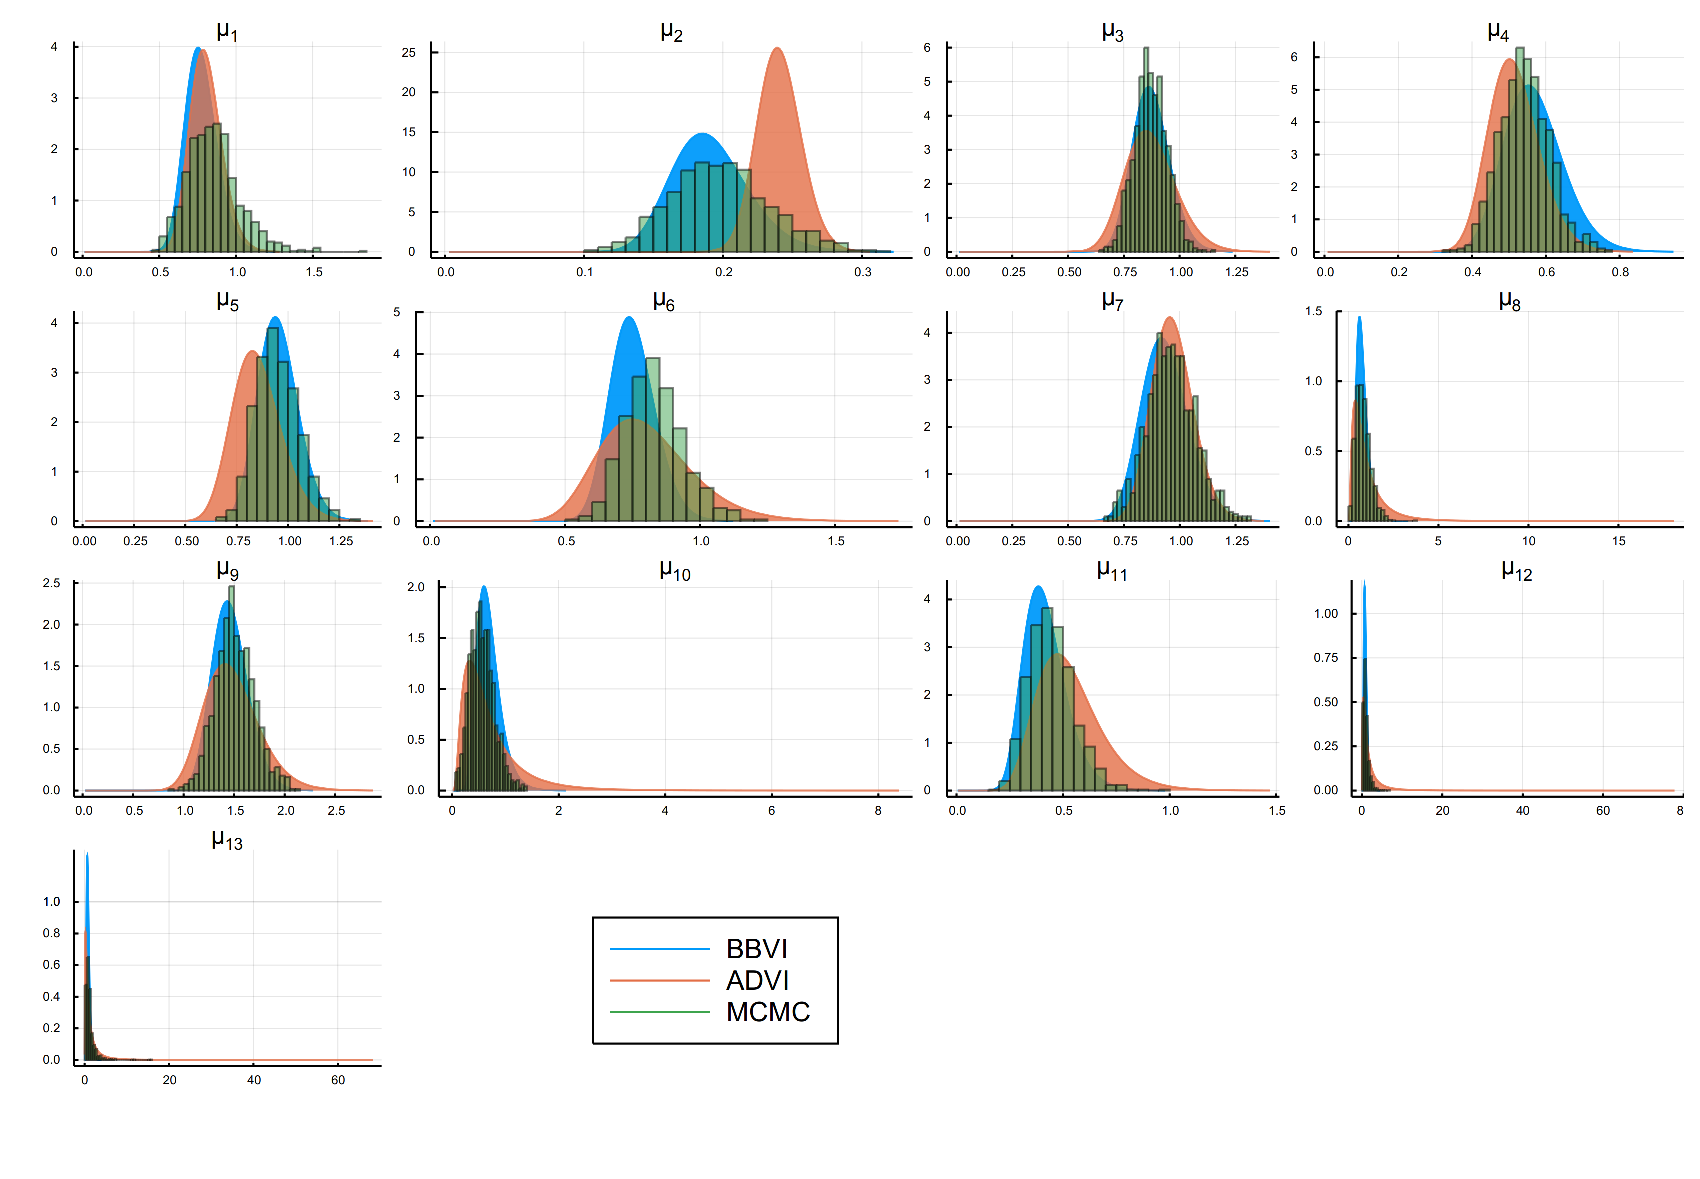
\includegraphics[width=6in]{images/whale/whale-distribution-mu.eps}
	\caption[Whale experiment $\mu$ distributions.]{Comparison of different inference algorithms for the Whale model. The distributions of the different loss rates $\mu$ are given for BBVI (blue), ADVI (orange) and MCMC (green) respectively.}
    \label{fig:whale-mu}
\end{figure}


\section{Conclusions}
In general it is clear from the experiments that the variational approximations can serve as a substitute for MCMC in cases where computational speed is preferred or where researcher want to design studies with larger species trees. For the Beluga and Whale models discussed in this Chapter, BBVI is both the fastest and most similar to MCMC of the variational algorithms that were studied.
\chapter{Discussion}


\section{Discussion}

In this thesis we reviewed the potential of variational Bayesian inference for use with the statistical models currently being developed at the VIB.
\\
Bayesian inference with MCMC is computationally intensive and often requires that an analysis be performed on only a subset of the data. In the phylogenetic models discussed in this thesis, only 1000 gene families are used in the analysis, whereas typically between 8000 and 10.000 are available after pre-processing of the data. For the sake of computational expediency the species trees typically only contain around 10 species.
\medskip
\par In this thesis we showed that variational inference techniques can be applied to provide fast approximate inference with results that are directly comparable to MCMC in terms of accuracy. These methods are sufficiently fast to allow the design of larger studies and to use the full available dataset rather than having to subsample for computational reasons.

\medskip

\par In the simulation we found that BBVI best approximated the MCMC, and that SVGD is largely useless for the Beluga model, because the model gradient is too computationally expensive. Perhaps it would be better suited to models where the gradient is not much more expensive than the joint likelihood of the model. There may be cases where the model gradient can be explicitly computed (without AD), but this would largely defeat the purpose of using a generic variational algorithm. The experiment with the high-quality rice data showed similar results: BBVI again slightly outperformed ADVI and was a bit faster. We found low duplication and loss rates in most of the branches, which is to be expected from closely related species.

\medskip

\par It is however unclear why the results of the PLAZA experiment lead to such tiny values for the duplication and loss rates. Perhaps this is because not enough data was used (only 250 gene families), a because of a mistake in the filtering of the data, or because the wrong prior was set. For computational reasons it was impossible to repeat the experiment with one of these factors modified. This should be investigated further in order to prove the validity of VI studies on larger species trees.

\medskip

\par The Whale experiment again demonstrated that BBVI was the most accurate method, and best approximated the MCMC gold standard. We note that when it comes to the WGD hypotheses, the differences between the ADVI result and MCMC are large enough for a researcher to draw a different conclusion from the two analyses. 

\medskip

\par From the experiments it appears that BBVI is a clear overall winner among the variational algorithms: it is both faster than ADVI and SVGD and more accurately approximates the MCMC gold standard. This is mainly because the BBVI does not use the model gradient and as such can use more MC samples without great computational cost.

\section{Future work}
The variational algorithms described in this thesis are those variants of the original algorithms that are currently used in other statistical packages. There exist more advanced variants of these methods in the academic literature which have been shown to be promising but have not yet been adopted by end users. There are variants of BBVI that use importance sampling and have been shown to improve convergence (\cite{bbvi-advances}).
\medskip
\par In this thesis the variational algorithms were limited to the mean-field normal variational family. While this is a strict limitation, the problems studied here deal mostly with latent variables that have lognormal distributions. The normal variational distribution in real-space becomes a lognormal after transforming with a transformation $\mathrm{T}$ so in this case the mean-field normal family is a very good choice. This may not be so for other phylogenetic models, so the effect of more complex variational families is something that should be studied more closely. 
\medskip
\par In addition to the uses demonstrated in this thesis, VI can also be applied for model selection, as the ELBO is an estimator for the marginal likelihood \cite{19}. The ELBO could then be used to determine which of two models best fits the data. For example, calculating the optimal ELBO (e.g. with BBVI) for two
models using different species. If the models are optimised with the same data then we could say that the model with the largest ELBO fits the data best; and as a result that its species tree better represents the phylogenetic data.

\section{Conclusion}
\par In general, it is clear that variational inference will come to play a larger role in bioinformatics in this age of Big Data, where more and more high-quality genomes are available and researchers want to design ever larger studies. 

% Materials and methods

\chapter{Methods and materials}

\section{Variational algorithms}
The implementation of the variational inference algorithms of BBVI, ADVI and SVGD used in the experiments are available at \textit{https://github.com/savmasse/PhyloVI}. These implementations are identical to how they are described in the original papers (see Chapter \ref{sec:vi}), except that we chose to use the ADAM optimiser instead of the different optimisation algorithms that each paper suggests.

\section{Phylogenetic models}


\subsection{Beluga \parencite{beluga}}
Beluga is a phylogenetic inference library that models the evolutionary history of a set of species with duplication and loss rates in each branch. All analyses in this thesis were performed with the  \textit{IidRevJumpPrior} prior as implemented in the Beluga library, each time using the exact same prior for VI and MCMC. The experiments were performed on a now outdated version of Beluga (commit \textit{92f2ab4ce4bc6df383a85f16666fd84d7d6d7f37} on the master branch). The MCMC algorithm used in the Beluga model was a reversible jump algorithm.
 
\subsection{Whale \parencite{whale}}
Whale.jl is a phylogenetic inference library that similarly describes the history of a species tree in terms of duplications, losses and larger whole genome duplication events. Experiments were performed on the mul branch of Whale as it stands at the time of writing (commit \textit{fbc0cc84ab9ae90efcec6c849ae76685a73d5a8e}) . This version of Whale used Hamiltonian Monte Carlo as its MCMC algorithm.


\section{Data}

In this section the origin and preprocessing of the data is discussed. If an experiment from Chapter \ref{sec:results} is not mentioned here that means the data was obtained as-is from my supervisor, and the exact pre-processing steps used could not be determined.


\subsection{Rice dataset}
\par
\medskip
\par The gene families used in the experiments using the Beluga model have always been filtered according to the following principle. Gene families that do not have at least one gene in the outgroup are filtered out. Additionally, those families that are extremely small (<10 genes) or extremely large (>100 genes) were also filtered out. 
\medskip
\par ADVI and BBVI were run for 1000 iterations with mini-batches of 100 samples, whereas the MCMC was run for 10,000 iterations (with 1000 burn-in) on the full dataset.

\subsection{PLAZA dataset}
The PLAZA dicot 4.0 dataset contains 55 plant species. However, not all of these species could be resolved into a noncontroversial bifurcating tree with the NCBI taxanomy browser \parencite{ncbi}; those that conflicted were dropped from the analysis, leaving 44 remaining species (Figure \ref{fig:PLAZA-trees}). The gene count data for the Beluga analysis was also obtained from the PLAZA database and filtered on gene family size (30<N<200).
\\ 
For computational reasons the data used in the experiment consists of a subset of only 250 gene families. The BBVI algorithm was run for 1000 iterations with mini-batches of 100 samples.

\subsection{Whale dataset}
The 500 ALE trees used in the Whale experiment were received from my supervisor and were already filtered. How the filtering was performed is unclear. Whale was run for 1000 iterations, while ADVI and BBVI were both run for 1000 iterations with mini-batches of 50 samples.


\section{Computational resources}
All computation times given in this document were obtained on a Dell XPS 15 (2018) with a i7-8750H CPU (2.2$\,$GHz base, 4.10$\,$GHz turbo), using all 6 cores in parallel. 

\section{Code availability}
The Julia code for the project is available at \textit{https://github.com/savmasse/PhyloVI}.  An export of the Overleaf LateX project code for this thesis document can be found at \\ \textit{https://github.com/savmasse/thesis-bioinformatics}.


% Lists
\clearpage

% Bibliography
%
\begin{thebibliography}{50}

\bibitem{PLAZA-site}
Website: https://bioinformatics.psb.ugent.be/plaza/, accessed on 24/04/2020

\bibitem{PLAZA-paper-1}
Van Bel, M., Diels, T., Vancaester, E., Kreft, L., Botzki, A., Van de Peer, Y., Coppens, F., Vandepoele, K. (2017) PLAZA 4.0: an integrative resource for functional, evolutionary and comparative plant genomics Nucleic Acids Res.

\bibitem{PLAZA-paper-2}
Vandepoele, K., Van Bel, M., Richard, G., Van Landeghem, S., Verhelst, B., Moreau, H., Van de Peer, Y., Grimsley, N., Piganeau, G. (2013) pico-PLAZA, a genome database of microbial photosynthetic eukaryotes. Environmental Microbiology 15(8):2147-53

\bibitem{ADVI}
Kucukelbir, Alp \& Tran, Dustin \& Ranganath, Rajesh \& Gelman, Andrew \& Blei, David. (2016). Automatic Differentiation Variational Inference. 18. 

\bibitem{ADVI-stan}
Kucukelbir, A., Tran, D., Ranganath, R., Gelman, A., \& Blei, D. M. (2017). Automatic differentiation variational inference. The Journal of Machine Learning Research, 18(1), 430-474.

\bibitem{vi-review}
Blei, D. M., Kucukelbir, A., \& Mcauliffe, J. D. (2017). Variational Inference: A Review for Statisticians. Journal of the American Statistical Association, 112(518), 859-877. doi:10.1080/01621459.2017.1285773

\bibitem{svi-cat}
Dang, T., \& Kishino, H. (2018). Stochastic Variational Inference for Bayesian Phylogenetics: A Case of CAT Model. doi:10.1101/358747

\bibitem{BBVI}
Ranganath, R., Gerrish, S., \& Blei, D. (2014, April). Black box variational inference. In Artificial Intelligence and Statistics (pp. 814-822).

\bibitem{SVGD-website}
Website: http://www.cs.utexas.edu/~qlearning/project.html?p=svgd, accessed on 26/07/2020

\bibitem{SVGD}
Liu, Q., \& Wang, D. (2016). Stein variational gradient descent: A general purpose bayesian inference algorithm. In Advances in neural information processing systems (pp. 2378-2386).

\bibitem{KL}
Kullback, S.; Leibler, R. A. On Information and Sufficiency. Ann. Math. Statist. 22 (1951), no. 1, 79--86. doi:10.1214/aoms/1177729694. https://projecteuclid.org/euclid.aoms/1177729694

\bibitem{ADAM}
Kingma, D. P., \& Ba, J. (2014). Adam: A method for stochastic optimization. arXiv preprint arXiv:1412.6980.

\bibitem{Flux}
Innes, M., Saba, E., Fischer, K., Gandhi, D., Rudilosso, M. C., Joy, N. M., ... & Shah, V. (2018). Fashionable modelling with Flux. arXiv preprint arXiv:1811.01457.

\bibitem{Stan}
Carpenter, B., Gelman, A., Hoffman, M. D., Lee, D., Goodrich, B., Betancourt, M., ... & Riddell, A. (2017). Stan: A probabilistic programming language. Journal of statistical software, 76(1).

\bibitem{rice}
Stein, J.C., Yu, Y., Copetti, D. et al. Genomes of 13 domesticated and wild rice relatives highlight genetic conservation, turnover and innovation across the genus Oryza. Nat Genet 50, 285–296 (2018). https://doi.org/10.1038/s41588-018-0040-0

\bibitem{pymc3}
Salvatier J., Wiecki T.V., Fonnesbeck C. (2016) Probabilistic programming in Python using PyMC3. PeerJ Computer Science 2:e55 DOI: 10.7717/peerj-cs.55.

\bibitem{rice-split}
Thiel, T., Graner, A., Waugh, R., Grosse, I., Close, T. J., \& Stein, N. (2009). Evidence and evolutionary analysis of ancient whole-genome duplication in barley predating the divergence from rice. BMC evolutionary biology, 9, 209. https://doi.org/10.1186/1471-2148-9-209

\bibitem{AD}
Margossian, C. C. (2019). A review of automatic differentiation and its efficient implementation. Wiley Interdisciplinary Reviews: Data Mining and Knowledge Discovery, 9(4), e1305.

\bibitem{forwarddiff}
Revels, J., Lubin, M., & Papamarkou, T. (2016). Forward-mode automatic differentiation in Julia. arXiv preprint arXiv:1607.07892.

\bibitem{rao-blackwell}
Casella, G., & Robert, C. P. (1996). Rao-Blackwellisation of sampling schemes. Biometrika, 83(1), 81-94.

\bibitem{control-variate}
S. M. Ross. Simulation. Elsevier, 2002.

\bibitem{itol}
Ivica Letunic, Peer Bork, Interactive Tree Of Life (iTOL) v4: recent updates and new developments, Nucleic Acids Research, Volume 47, Issue W1, 02 July 2019, Pages W256–W259.

\bibitem{Turing}
Hong Ge, Kai Xu, Zoubin Ghahramani; Proceedings of the Twenty-First International Conference on Artificial Intelligence and Statistics, PMLR 84:1682-1690, 2018.

\bibitem{mrbayes}
Huelsenbeck, J. P., & Ronquist, F. (2001). MRBAYES: Bayesian inference of phylogenetic trees. Bioinformatics, 17(8), 754-755.

\bibitem{vi}
Beal, M. J. (2003). Variational algorithms for approximate Bayesian inference (Doctoral dissertation, UCL (University College London)).

\bibitem{bayes-ecology}
Ellison, A. M. (2004). Bayesian inference in ecology. Ecology letters, 7(6), 509-520.

\bibitem{vi-genome-environment}
Montesinos-López, O. A., Montesinos-López, A., Crossa, J., Montesinos-López, J. C., Luna-Vázquez, F. J., Salinas-Ruiz, J., Herrera-Morales, J. R., \& Buenrostro-Mariscal, R. (2017). A Variational Bayes Genomic-Enabled Prediction Model with Genotype × Environment Interaction. G3 (Bethesda, Md.), 7(6), 1833–1853. https://doi.org/10.1534/g3.117.041202

\bibitem{phylostan}
Fourment, M., & Darling, A. E. (2019). Evaluating probabilistic programming and fast variational Bayesian inference in phylogenetics. PeerJ, 7, e8272.

\bibitem{cat}
Dang, T., & Kishino, H. (2019). Stochastic variational inference for Bayesian phylogenetics: a case of CAT model. Molecular biology and evolution, 36(4), 825-833.

\bibitem{bbvi-advances}
Agrawal, A., Sheldon, D., & Domke, J. (2020). Advances in Black-Box VI: Normalizing Flows, Importance Weighting, and Optimization. arXiv preprint arXiv:2006.10343.

\bibitem{ncbi}
Sayers EW, Cavanaugh M, Clark K, Ostell J, Pruitt KD, Karsch-Mizrachi I. GenBank. Nucleic Acids Res. 2019 Jan 8;47(D1):D94-D99.

\bibitem{19}
Fourment, M., Magee, A. F., Whidden, C., Bilge, A., Matsen IV, F. A., \& Minin, V. N. (2020). 19 dubious ways to compute the marginal likelihood of a phylogenetic tree topology. Systematic Biology, 69(2), 209-220.


\end{thebibliography}
\printbibliography

% Appendix
\appendix
\chapter{Implementation}

\section{Notes on the state of the art}
At the start of this project there were no publicly available Julia packages that implemented the variational inference techniques studied here. However, since then there have been developments in the field. The Turing.jl package, a general-purpose probabilistic programming library, now has an ADVI implementation and plans to add others \parencite{Turing}; although this is not yet available in the current stable release version.

\section{Notes on the accompanying package PhyloVI}
A variational inference library written in the Julia language called PhyloVI is available on GitHub at \textit{www.github.com/savmasse/PhyloVI}. It contains all code relevant to this thesis project; both the implementation of the algorithms and the code used to generate the plots for this document. PhyloVI was written in Julia 1.3 and is not guaranteed to function in any other version of Julia.

\afterpage{\blankpage}
\includepdf[pages=1]{images/titelblad.pdf}

\end{document}
